\documentclass[a4paper,12pt]{report}

% Page layout
\usepackage[left=2.5cm,right=2.5cm,top=2.5cm,bottom=2.5cm]{geometry}

% Font and text
\usepackage[english]{babel}
\usepackage{microtype}
\usepackage{setspace}
\usepackage{lmodern}
\usepackage{siunitx}
\newcommand{\myemph}[1]{{\sffamily\bfseries#1}}
\sloppy
\onehalfspacing

% Headings
\usepackage[raggedright,sf,bf]{titlesec}
\usepackage[margin=\the\parindent,small,bf,sf]{caption}
\titlelabel{\thetitle.\ }
\titleformat{\chapter}[display]{\huge\bfseries\sffamily}{\chaptertitlename\ \thechapter}{15pt}{\Huge \raggedright}
\titlespacing*{\chapter}{0pt}{0pt}{40pt}  % remove spacing before chapter headings
\makeatletter
\let\originall@chapter\l@chapter
\def\l@chapter#1#2{\originall@chapter{{\sffamily #1}}{#2}}
\makeatother

%% Alternative headings using small-caps (comment out the top section)
%\usepackage[raggedright,bf]{titlesec}
%\usepackage[margin=\the\parindent,small,bf]{caption}
%\titlelabel{\thetitle.\ }
%\titleformat{\chapter}[display]{\huge\scshape}{\chaptertitlename\ \thechapter}{15pt}{\Huge \raggedright}
%\titlespacing*{\chapter}{0pt}{0pt}{40pt}  % remove spacing before chapter headings

% Table of contents
\let \savenumberline \numberline
\def \numberline#1{\savenumberline{#1.}}

% Figures
\usepackage{graphicx}
% \usepackage{grffile}
\usepackage{pdfpages}
\usepackage{subcaption}
\setlength{\abovecaptionskip}{7.5pt}  % spacing above and below captions
\newcommand*{\WaterMark}[2][0.2\paperwidth]{\AddToShipoutPicture*{\AtTextCenter{\parbox[c]{0pt}{\makebox[0pt][c]{\includegraphics[width=#1]{#2}}}}}}

% Mathematics
\usepackage[cmex10]{amsmath}
\usepackage{amssymb}
\usepackage{cancel}
\DeclareMathOperator*{\argmax}{arg\,max}
\newcommand{\T}{^\top}
\newcommand{\tr}{\textrm{tr}}
\renewcommand{\vec}[1]{\boldsymbol{\mathbf{#1}}}
\newcommand{\defeq}{\triangleq}

% Tables
\usepackage{booktabs}
\usepackage{tabularx}
\usepackage{multirow}
\newcommand{\mytable}{
    \centering
    \small
    \renewcommand{\arraystretch}{1.2}
    }
\renewcommand{\tabularxcolumn}[1]{m{#1}}
\newcolumntype{C}{>{\centering\arraybackslash}X}
\newcolumntype{L}{>{\raggedright\arraybackslash}X}

% Header and footer
\usepackage{fancyhdr}
\pagestyle{fancy}
\fancyhf{}
\renewcommand{\sectionmark}[1]{\markright{\normalsize \thesection.\ #1}}
\fancyhead[C]{\nouppercase{\textit{\rightmark}}}
\fancyhead[RO]{\thepage}
\fancyhead[LE]{\thepage}  % double-sided printing
\fancyfoot{}
\setlength\headheight{14.5pt}
\renewcommand{\headrulewidth}{0pt}
\fancypagestyle{plain}{\fancyhead{}
                       \renewcommand{\headrulewidth}{0pt}
                       \fancyfoot[C]{\thepage}}

% Pseudo-code
\usepackage{algorithm}  % should go before \usepackage{hyperref}

% Table of contents and hyperlinks
\usepackage{hyperref}
\hypersetup{colorlinks=true,linktoc=all,citecolor=black,linkcolor=black}
\usepackage[nottoc]{tocbibind}

% Pseudo-code
\usepackage{algpseudocode}  % should go after \usepackage{hyperref}
\renewcommand{\thealgorithm}{\arabic{chapter}.\arabic{algorithm}} 
\captionsetup[algorithm]{labelfont={bf,sf},font=small,labelsep=colon}

% Bibliography
\usepackage{cite}  % automatically reorder inline citations
\bibliographystyle{IEEEtran}
\bibliography{IEEEabrv, mybib}

% Fix titlesec issue
\usepackage{etoolbox}
\makeatletter
\patchcmd{\ttlh@hang}{\parindent\z@}{\parindent\z@\leavevmode}{}{}
\patchcmd{\ttlh@hang}{\noindent}{}{}{}
\makeatother

\DeclareUnicodeCharacter{2212}{-}

\begin{document}

% Front matter
\graphicspath{{frontmatter/fig/}}
\pagenumbering{Alph}

\begin{titlepage}
	\begin{center}
		
		
\includegraphics[width=10cm]{USlogo-top}
		
		\vfill
		
		{\sffamily \bfseries \huge A Critical Analysis of Design Flaws in the Death Star \par}
%		{\scshape \huge A Critical Analysis of Design Flaws in the Death Star \par}
		
		\vfill
		
		{\large {\Large Luke Skywalker} \\ 99652154 \par}
		
		\vfill
		
		\vfill
		
		{Report submitted in partial fulfilment of the requirements of the module \\
			Project (E) 448 for the degree Baccalaureus in Engineering in the Department of
			Electrical and Electronic Engineering at Stellenbosch University. \par}
		
		\vfill
		
		{\large {Supervisor}: Dr O.\ W.\ Kenobi} %\\
		% Department of Electrical and Electronic Engineering \par}
		
		\vfill
		
		{\Large October 2099}
	\end{center}
\end{titlepage}

%\graphicspath{{frontmatter/fig/}}
\pagenumbering{Alph}

\begin{titlepage}
	\begin{center}
		
		%
\includegraphics[width=10cm]{USlogo-top}
		
		\WaterMark{UScrest-WM}
		
		~\vspace{4.5em}
		
		{\sffamily \bfseries \huge A Critical Analysis of Design Flaws in the Death Star \par}
%		{\scshape \huge A Critical Analysis of Design Flaws in the Death Star \par}		
		
		\vspace{7em}
		
		{\large {\Large  Luke Skywalker} \\ 99652154 \par}
		
		\vspace{8em}
		
		{\large Thesis presented in partial fulfilment of the requirements for the degree of \\ Master of Engineering (Electronic) in the Faculty of Engineering at Stellenbosch University. \par}
		
		\vfill
		
		{\large {Supervisor}: Dr O.\ W.\ Kenobi\\
		Department of Electrical and Electronic Engineering \par}
		
		%\vfill
		\vspace{10em}
		
		{\Large October 2099}
	\end{center}
\end{titlepage}

\pagenumbering{roman}
\chapter*{Acknowledgements}
% \addcontentsline{toc}{chapter}{Acknowledgements}
\makeatletter\@mkboth{}{Acknowledgements}\makeatother

I would like to thank my dog, Muffin. I also would like to thank the inventor of the incubator; without him/her, I would not be here. Finally, I would like to thank Dr Herman Kamper for this amazing report template.
%\chapter*{Declaration}
\newpage
\thispagestyle{plain}
\addcontentsline{toc}{chapter}{Declaration}
\makeatletter\@mkboth{}{Declaration}\makeatother

\centerline{
\includegraphics[width=8cm]{USlogo-top}}
\vspace*{-10pt}

\section*{\centering Plagiaatverklaring / \textit{Plagiarism Declaration}}

\vspace*{5pt}

\begin{enumerate}
    \item Plagiaat is die oorneem en gebruik van die idees, materiaal en ander intellektuele eiendom van ander persone asof dit jou eie werk is.\\
    \textit{Plagiarism is the use of ideas, material and other intellectual property of another's work
        and to present is as my own.}
    
    \item Ek erken dat die pleeg van plagiaat 'n strafbare oortreding is aangesien dit 'n vorm van diefstal is.\\
    \textit{I agree that plagiarism is a punishable offence because it constitutes theft.}
    
    \item Ek verstaan ook dat direkte vertalings plagiaat is. \\
    \textit{I also understand that direct translations are plagiarism.}
    
    \item Dienooreenkomstig is alle aanhalings en bydraes vanuit enige bron (ingesluit die internet) volledig verwys (erken). Ek erken dat die woordelikse aanhaal van teks sonder aanhalingstekens (selfs al word die bron volledig erken) plagiaat is. \\
    \textit{Accordingly all quotations and contributions from any source whatsoever (including the internet) have been cited fully. I understand that the reproduction of text without quotation marks (even when the source is cited) is plagiarism}
    
    \item Ek verklaar dat die werk in hierdie skryfstuk vervat, behalwe waar anders aangedui, my eie oorspronklike werk is en dat ek dit nie vantevore in die geheel of gedeeltelik ingehandig het vir bepunting in hierdie module/werkstuk of 'n ander module/werkstuk~nie. \\
    \textit{I declare that the work contained in this assignment, except where otherwise stated, is my original work and that I have not previously (in its entirety or in part) submitted it for grading in this module/assignment or another module/assignment.}
\end{enumerate}

\vfill

\noindent \begin{tabularx}{1.0\linewidth}{|L|L|}
    \hline
    \vspace{1cm} {Studentenommer / \textit{Student number}} & \vspace{1cm} {Handtekening / \textit{Signature}} \\
    \hline
    \vspace{1cm} {Voorletters en van / \textit{Initials and surname}} & \vspace{1cm} {Datum / \textit{Date}} \\
    \hline
\end{tabularx}

\vspace{15pt}

% The old declaration

%I, the undersigned, hereby declare that the work contained in this report is my own original work unless otherwise stated.
%
%% Afrikaans:
%% Hiermee verklaar ek, die ondergetekende, dat die werk in hierdie verslag vervat my eie oorspronklike werk is, tensy anders vermeld.
%
%\vspace{2.5cm}
%
%\begin{table}[h]
%\begin{tabular}{@{}p{2.5cm}p{5cm}}
%    Signature: & \dotfill \\
%    & \multicolumn{1}{c}{Obi-Wan Kenobi} \\
%    ~\vspace{1cm} \\
%    Date: & \dotfill \\
%\end{tabular}
%\end{table}
%
%\vfill
%
%\begin{center}
%    Copyright \textcopyright\ 2099 Stellenbosch University \\
%    All rights reserved
%\end{center}


\chapter*{Abstract}
\addcontentsline{toc}{chapter}{Abstract}
\makeatletter\@mkboth{}{Abstract}\makeatother

\subsubsection*{English}

The English abstract.

\selectlanguage{english}
\tableofcontents
\listoffigures
\listoftables
\chapter*{Nomenclature\markboth{}{Nomenclature}}
\addcontentsline{toc}{chapter}{Nomenclature}

% % \vspace*{-3mm}
% \subsubsection*{Variables and functions}

% \begingroup
% \renewcommand{\arraystretch}{1.2}
% \renewcommand{\tabularxcolumn}[1]{p{#1}}
% \begin{tabularx}{\textwidth}{@{}p{2.5cm}L}
%     $p(x)$ & Probability density function with respect to variable $x$.\\
%     $P(A)$ & Probability of event $A$ occurring.\\
%     $\varepsilon$ & The Bayes error. \\
%     $\varepsilon_u$ & The Bhattacharyya bound. \\
%     $B$ & The Bhattacharyya distance. \\
%     $s$ & An HMM state.  A subscript is used to refer to a particular state, e.g.\ $s_i$ refers to the $i^{\text{th}}$ state of an HMM. \\
%     $\mathbf{S}$ & A set of HMM states. \\
%     $\mathbf{F}$ & A set of frames. \\
%     $\mathbf{o}_f$ & Observation (feature) vector associated with frame $f$. \\
%     $\gamma_s(\mathbf{o}_f)$ & A posteriori probability of the observation vector $\mathbf{o}_f$ being generated by HMM state $s$. \\
%     $\mu$ & Statistical mean vector. \\
%     $\Sigma$ & Statistical covariance matrix. \\
%     $L(\mathbf{S})$ & Log likelihood of the set of HMM states $\mathbf{S}$ generating the training set observation vectors assigned to the states in that set. \\
%     $\mathcal{N}(\mathbf{x} | \mu, \Sigma)$ & Multivariate Gaussian PDF with mean $\mu$ and covariance matrix $\Sigma$.\\
%     $a_{ij}$ & The probability of a transition from HMM state $s_i$ to state $s_j$. \\
%     $N$ & Total number of frames or number of tokens, depending on the context. \\
%     $D$ & Number of deletion errors. \\
%     $I$ & Number of insertion errors. \\
%     $S$ & Number of substitution errors. \\
% \end{tabularx}
% \endgroup


% \newpage
\subsubsection*{Acronyms and abbreviations}

\begingroup
\renewcommand{\arraystretch}{1.2}
\begin{tabular}{@{}p{2.5cm} l}
    $USV$ & Unmanned Sailing Vessel. \\
    $GPS$ & Global Positioning System. \\
    $RC$ & Radio Controlled \\
    $CAD$ & Computer Aided Design \\
    $P controller$ & Proportional controller \\
    $PI$ & Proportional Integral \\
    $PID$ & Proportional Integral Derivative \\
    $FPGA$ & Field Programmable Gate Array \\
    $SPI$ & Serial Peripheral Interface \\
    $IMU$ & Inertial Measurement Unit \\
    $PWM$ & Pulse Width Modulation \\
    $NMEA$ & \\
    $ASCII$ & American Standard Character for Information and Interchange \\
    $ADC$ & Analog to Digital Converter \\
    $UART$ & \\
    $PWM$ & Pulse Width Modulation \\   
    $FAT32$ & File Allocation Table, 32 bits \\
    $LSB$ & Least Significant Bit \\
    % AE      & Afrikaans English \\
    % AID     & accent identification \\
    % ASR     & automatic speech recognition \\
    % AST     & African Speech Technology \\
    % CE      & Cape Flats English \\
    % DCD     & dialect-context-dependent \\
    % DNN		& deep neural network \\
    % G2P     & grapheme-to-phoneme \\
    % GMM     & Gaussian mixture model \\
    % HMM     & hidden Markov model \\
    % HTK     & Hidden Markov Model Toolkit \\
    % IE      & Indian South African English \\
    % IPA     & International Phonetic Alphabet \\
    % LM      & language model \\
    % LMS     & language model scaling factor \\
    % MFCC    & Mel-frequency cepstral coefficient \\
    % MLLR    & maximum likelihood linear regression \\
    % OOV     & out-of-vocabulary \\
    % PD      & pronunciation dictionary \\
    % PDF     & probability density function \\
    % SAE     & South African English \\
    % SAMPA   & Speech Assessment Methods Phonetic Alphabet \\
\end{tabular}
\endgroup

\newpage
\pagenumbering{arabic}

% Contents
\graphicspath{{introduction/fig/}}

\chapter{Introduction}
\label{chap:introduction}

\section{Background}
The ocean covers 71$\%$ of the earths surface and 80$\%$ of it remains unmapped, unobserved, and unexplored. The ocean produces over half of the air we 
breathe and absorbs 50 times more carbon dioxide than our atmosphere currently does. It regulates our climate and the weather patterns by transporting heat
 from the equator to the poles. It provides sustenance to millions of people around the world. Many medicinal products that help to fight cancer, arthritis
  and heart disease come from the ocean. Marine transportation makes up a huge portion of global trade, which supports the economies of the world. Without 
  the ocean, life as we know it would not be possible and the planet would become uninhabitable.

The rapidly growing global population and consequent resource consumption is impacting the local and global environment negatively through physical and 
chemical pollution. The release of carbon dioxide into the atmosphere contributes to climate change, ocean warming, ocean acidification and the rise in sea
 levels. When released into the ocean, chemical wastes such agricultural fertilizers result in ocean deoxygenation. Many other forms of pollution such as 
 untreated waste water and micro and macro plastics have an environmental impact that as of yet is only partially known.

Ocean research has led to our current understanding of the huge role the oceans play in supporting life on this planet. The continuing research and 
exploration of our oceans will aid in assessing the growing negative impact human activity has on the oceans, and by better understanding this impact, 
more effective solutions can be developed. Ocean research requires large amounts of funding and human resources to support it. As of 2015 the United States 
had 4000 ocean science researchers, roughly 50 nationally maintained ocean research vessels and in 2013 had an annual national ocean science expenditure of
$\$12.5$ trillion \cite{Valdes}. These ocean research vessel cost from $\$10000$ to $\$40000$ a day to operate, with the crew itsef being one of the biggest 
expenses\cite{Valdes}.These expenses can increase greatly when research missions to remote areas of the globe are conducted, many of these areas being hard 
or even impossible to access via research vessels. 

Advancements in robotics and the development of unmanned vehicles can help bring down the cost and complexity associated with ocean research missions 
as well as increase the quality of research done. Unmanned sailing vessels(USV) will be able to travel long distances over the ocean, for long periods of 
time, to remote and inaccesable locations and with little power consumption. USV's can be equipped with various high quality sensors 
such as hydrophones that are used in marine research. The integration of solar panels with USV's can further increase the range and 
duration they are capable of.

\section{Problem Statement}
To design and develop the navigational and control systems for an unmanned sailing vessel that will enable it to sail along a predetermined route with a 
relative degree of accuracy. The route to be travelled is defined by a set of GPS coordinates. 

\section{Objectives}
This section will state the objectives that need to be achieved in order to address the problem statement.

In order for the navigational systems to work the following objectives need to be achieved. The USV should receive the current GPS coordinates with the 
standard degree of accuracy associated with the GPS, which is 2.5m. The USV 
should also be capable of logging the current GPS location as it travels along the route, this is needed to verify successful operation of the USV. 
Additionally the USV needs to calculate distance between two GPS cordinates accurately in order to determine when it has reached its target location. 
The USV should be able to calculate bearing given two GPS locations - its current GPS location and its target GPS location.


In order for the control systems to be work the following needs to be achieved.
The USV needs to be capable of measuring its current bearing to a relative degree of accuracy, this is a requirement for designing the rudder control system. 
The USV must be capable of determining wind direction relative to itself and adjust the sail position accordingly. 
The USV must be able to sail between two predetermined GPS coordinates with minimal deviation between its bearing and the bearing between the two coordinates.
The Vessel should be able to tack into the wind in order to reach a target location. Given that these two objectives have been achieved, the vessel should be
able to travel between three GPS coordinates such that the travelled path is a triangle.

\section{Summary of Work}

\section{Scope}



% \section{Section heading}

% This is some section with two table in it: Table~\ref{tbl:exemplars} and Table~\ref{tbl:abx_speaker}.

% \begin{table}[!h]
%     \mytable
%     \caption{Performance of the unconstrained segmental Bayesian model on TIDigits1 over iterations in which the reference set is refined.}
%     \begin{tabularx}{\linewidth}{@{}lCCCCC@{}}
%         \toprule
%         Metric     & 1 & 2 & 3 & 4 & 5 \\
%         \midrule
%         WER (\%)                        & $35.4$ & $23.5$ & $21.5$ & $21.2$ & $22.9$ \\
%         Average cluster purity (\%)       & $86.5$ & $89.7$ & $89.2$ & $88.5$ & $86.6$ \\
%         Word boundary $F$-score (\%)         & $70.6$ & $72.2$ & $71.8$ & $70.9$ & $69.4$ \\
%         Clusters covering 90\% of data   & 20             & 13 & 13 & 13 & 13 \\
%         \bottomrule
%     \end{tabularx}
%     \label{tbl:exemplars}
% \end{table}


% \begin{table}[!h]
%     \renewcommand{\arraystretch}{1.1}
%     \centering
%     \caption{A table with an example of using multiple columns.}
%     \begin{tabularx}{0.65\linewidth}{@{}lCCr@{}}
%         \toprule
%         & \multicolumn{2}{c}{Accuracy (\%)} \\
%         \cmidrule(lr){2-3}
%         Model    & Intermediate & Output & Bitrate\\
%         \midrule
%         Baseline & 27.5         & 26.4   & 116 \\
%         VQ-VAE   & 26.0         & 22.1   & 190 \\
%         CatVAE   & 28.7         & 24.3   & 215 \\
%         \bottomrule
%     \end{tabularx}
%     \label{tbl:abx_speaker}
% \end{table}

% \newpage

% This is a new page, showing what the page headings looks like, and showing how to refer to a figure like Figure~\ref{fig:cae_siamese}.

% \begin{figure}[!t]
%     \centering
% %     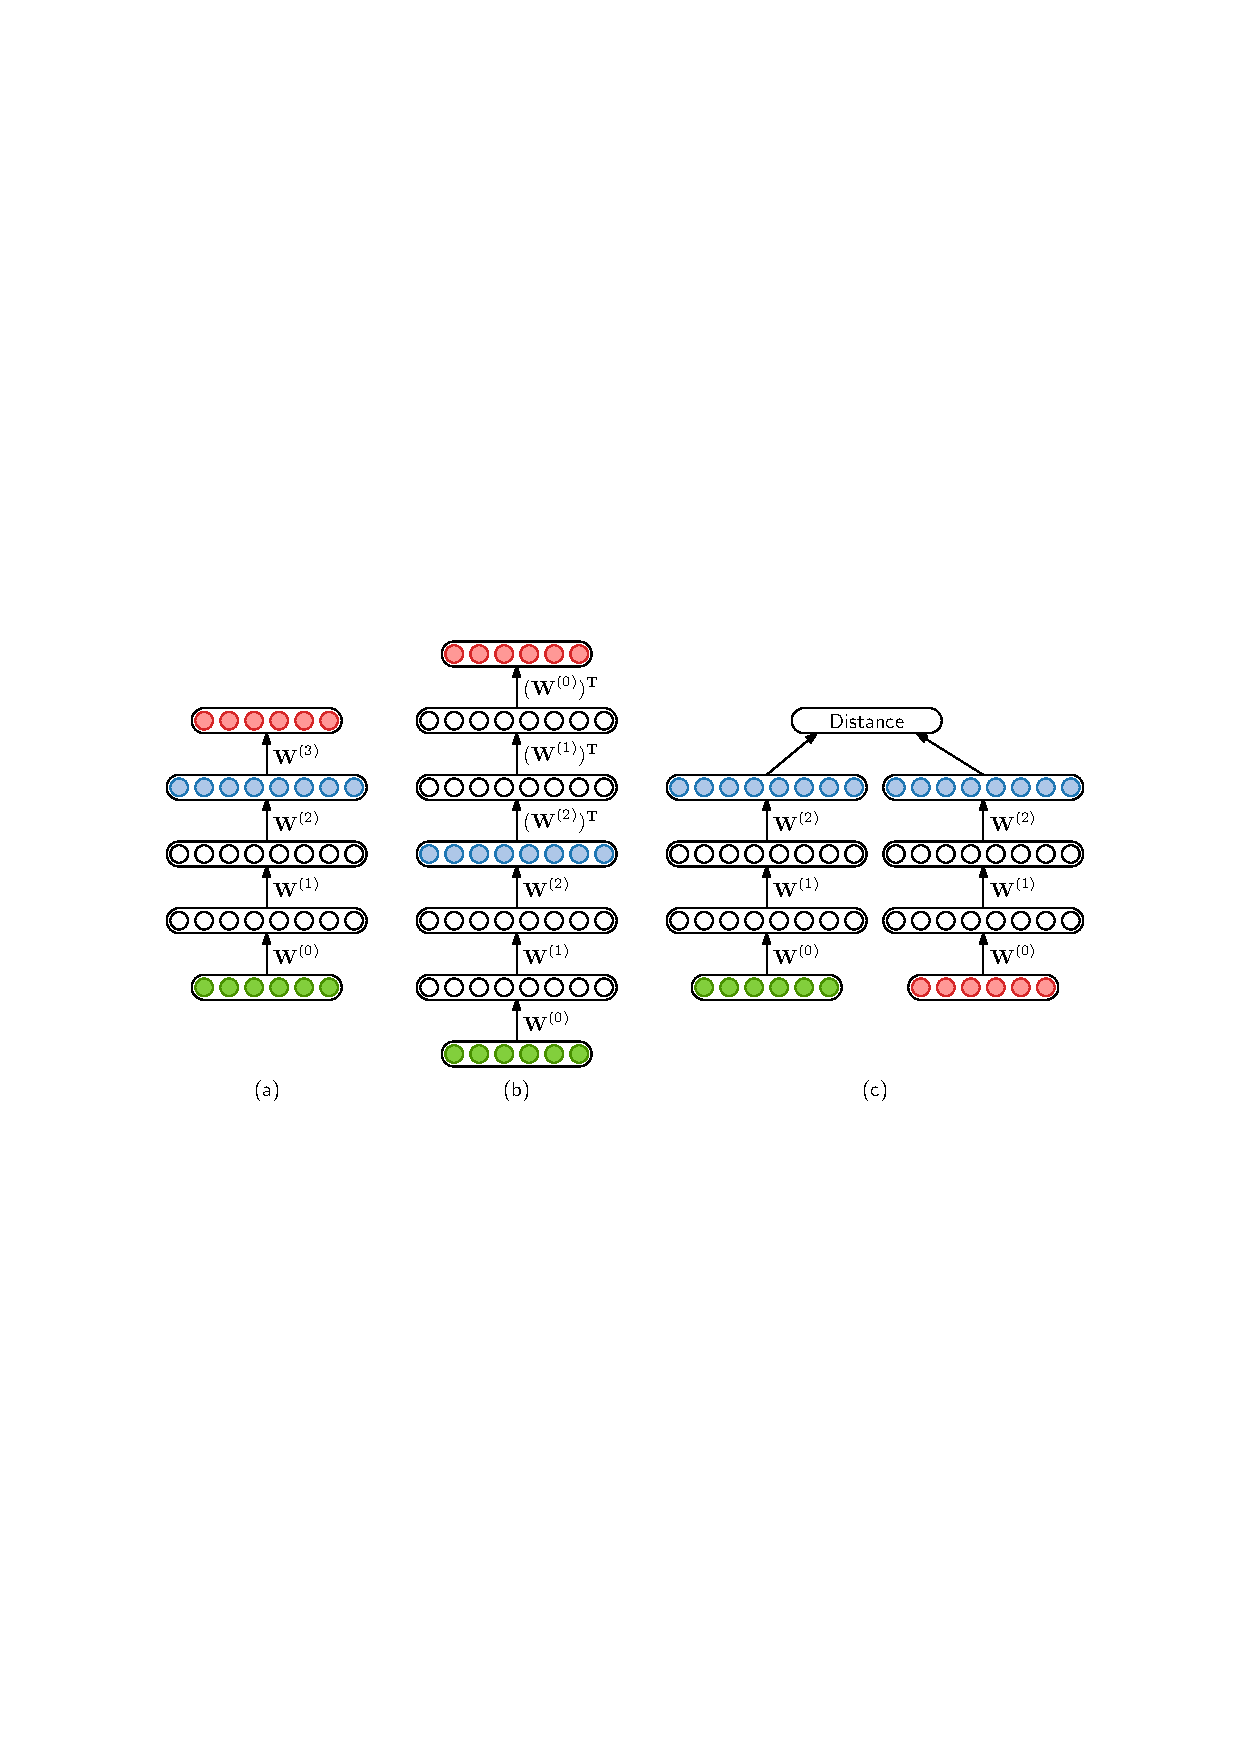
\includegraphics[width=\linewidth]{cae_siamese}
%     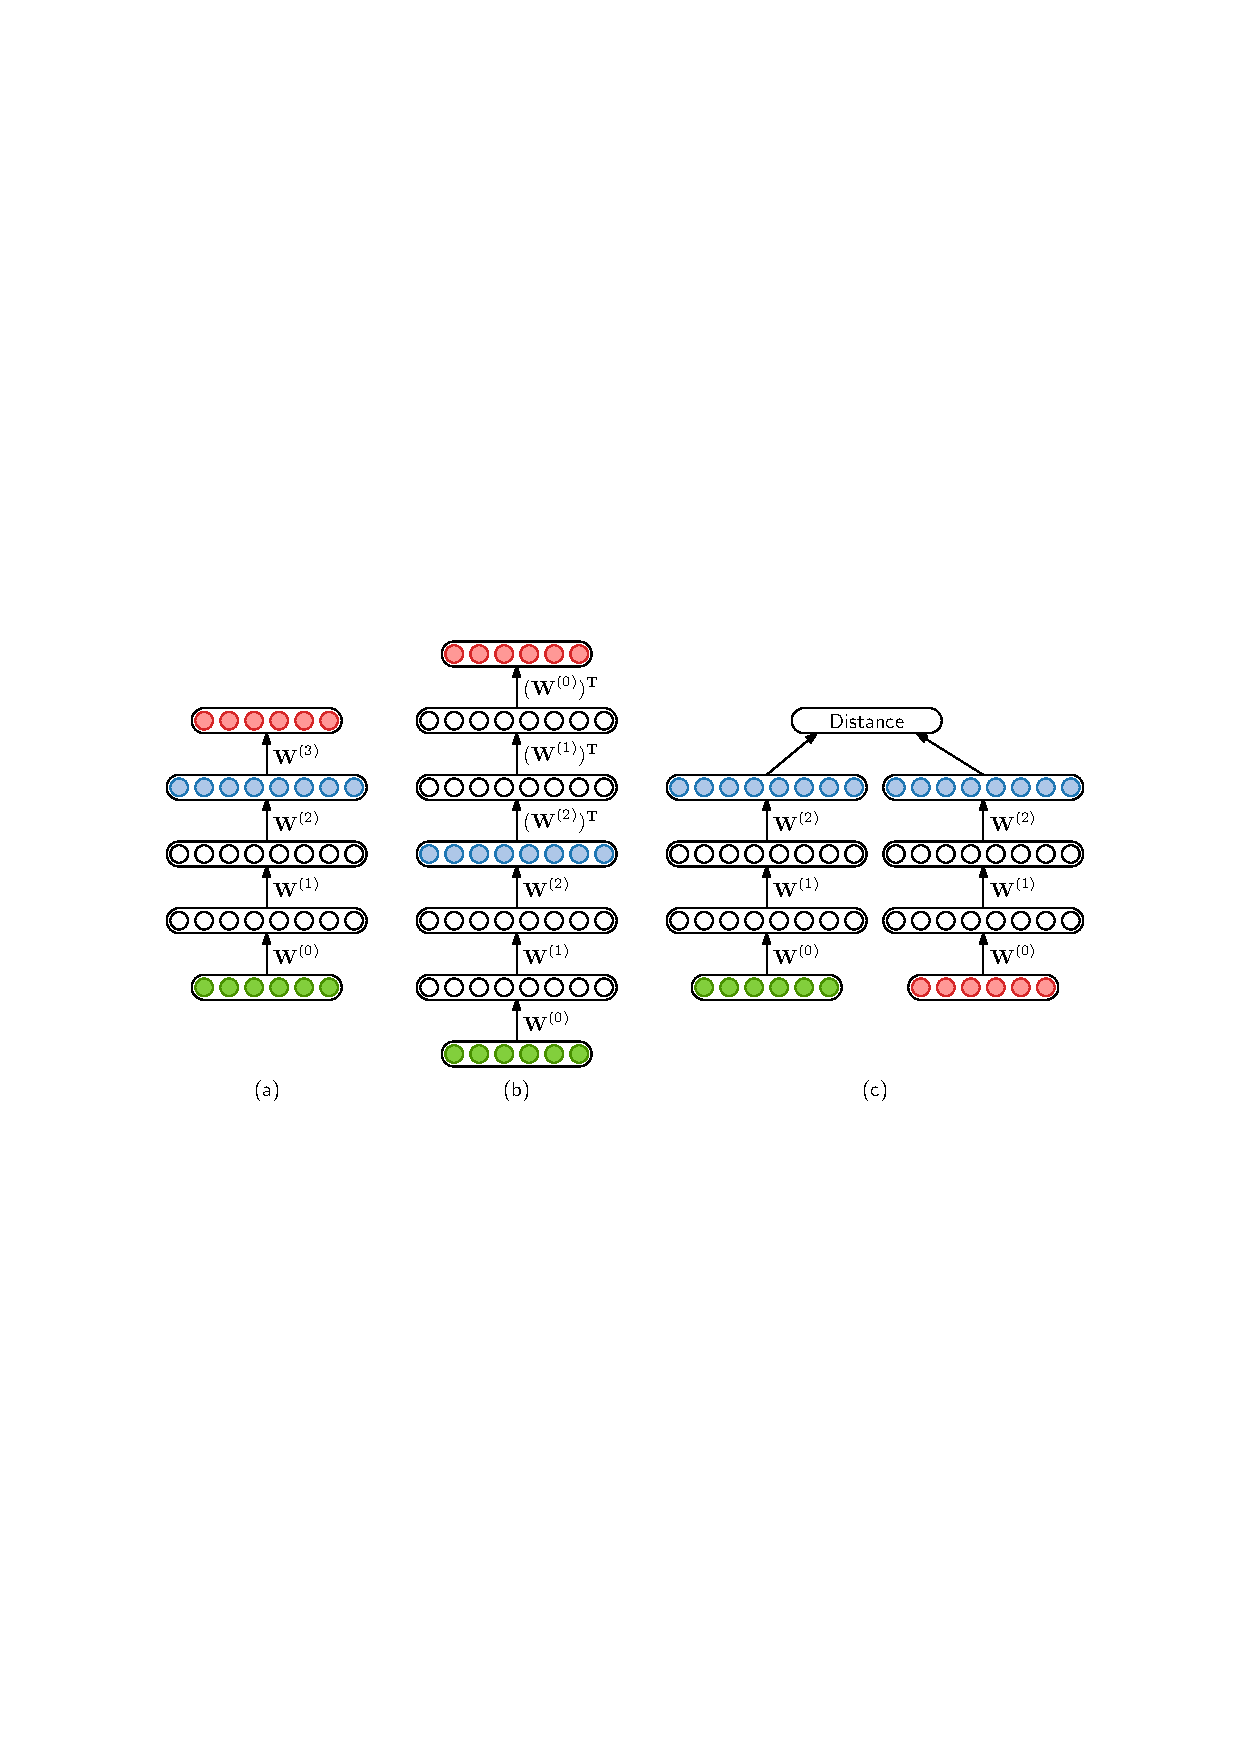
\includegraphics[width=0.918\linewidth]{cae_siamese}
%     \caption[I am the short caption that appears in the list of figures, without references.]{
%     (a) The cAE as used in this chapter. The encoding layer (blue) is chosen based on performance on a development set.
%     (b) The cAE with symmetrical tied weights. The encoding from the middle layer (blue) is always used.
%     (c) The siamese DNN. The cosine distance between aligned frames (green and red) is either minimized or maximized depending on whether the frames belong to the same (discovered) word or not.
%     A cAE can be seen as a type of DNN~\cite{dahl+etal_taslp12}.
%     }
%     \label{fig:cae_siamese}
% \end{figure}


% The following is an example of an equation:
% \begin{equation}
% P(\vec{z} | \vec{\alpha}) = \int_{\vec{\pi}} P(\vec{z} | \vec{\pi}) \, p(\vec{\pi} | \vec{\alpha}) \, \textrm{d} \vec{\pi}
% = \int_{\vec{\pi}} \prod_{k = 1}^K \pi_k^{N_k} \frac{1}{B(\vec{\alpha})} \prod_{k = 1}^K \pi_k^{\alpha_k - 1} \, \textrm{d} \vec{\pi}
% \label{eq:example_equation}
% \end{equation}
% which you can subsequently refer to as~\eqref{eq:example_equation} or Equation~\ref{eq:example_equation}.
% But make sure to consistently use the one or the other (and not mix the two ways of referring to equations).
\graphicspath{{literature/fig/}}

\chapter{Literature}

\section{Sail Theory}
This section covers the sailing theory that is required for the sections that follow, and is taken from the official manual of the american sailing 
association\cite{ASA}. Fig. \ref{fig:sailboat_anatomy} illustrates the anatomy of a typical sailboat. The anatomy of a sailboat is as follows:

\begin{itemize}
    \item Hull: Watertight floating body of the sailboat that gives it form and supports all parts of the part.
    \item Keel: Fixed fin on the underside of the sailboat that provides sideways resistance needed to counter the force of the wind on the sails.
    \item Stern: The back-end of the sailboat.
    \item Bow: The front-end of the sailboat
    \item Starboard: When standing at the stern, facing the bow, starboard is the right side of the boat.
    \item Port: When standing at the stern, facing the bow, port is the left side of the boat 
    \item Rudder: Fin located beneath the stern. The angle of the rudder is adjusted to steer the direction of the sailboat.
    \item Helm: The mechanism by which the rudder angle is adjusted.
    \item Mast: Vertical beam attached to the hull which houses the mainsail
    \item Mainsail: Sail that attaches to the mast of the sailboat.
    \item Jib: sail that attaches to the bow and the top of the mast.
\end{itemize}

\begin{figure}[!h]
    \centering
    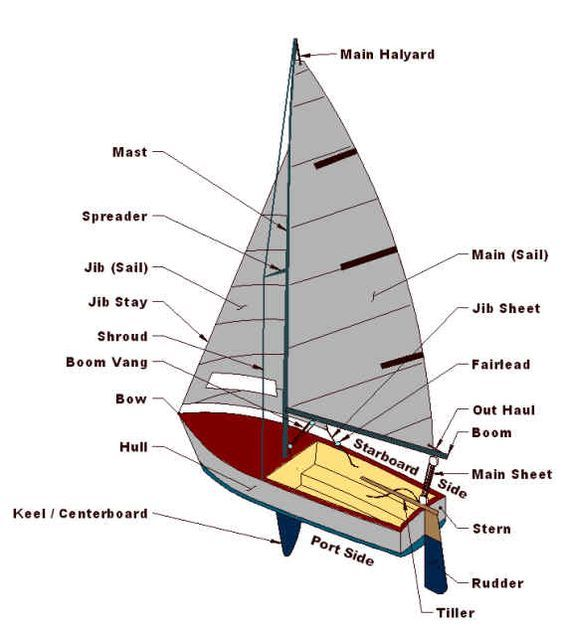
\includegraphics[width=0.6\linewidth]{sailboat_anatomy_1}
    \caption[Sailboat anatomy]{Sailboat anatomy \cite{sail_anatomy}}
    \label{fig:sailboat_anatomy}
\end{figure}

When on a sailboat the direction of the wind relative to the boat is known as the apparent wind, the direction of the wind relative to a fixed point - 
a point that has a zero velocity - is known as true wind. When the sailboat has a velocity that is not zero - sailboat not standing still - the apparent 
wind has a velocity that differs from the velocity of true wind. Fig. \ref{apparent_wind} illustrates this concept. 

\begin{figure}
    \centering
    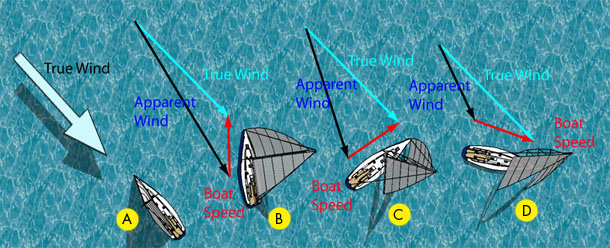
\includegraphics[width=0.7\linewidth]{apparent_wind.jpeg}
    \caption[Apparent wind]{Apparent wind\cite{apparent_wind} }
    \label{fig:apparent_wind}
\end{figure}


The sail of a sailboat acts similar to that of a airplane wing - it produces lift when orientated correctly. It is this lift that propels the sailboat 
forward. The orientation of the sail relative to the apparent wind therefore determines how much force is applied to the boat, any component of this force
that acts perpendicular to the centerline of the boat is canceled by the apposing force of the water on the keel. The act of changing the orientation of 
the sails is know as 'trimming the sails'. To generate a maximum amount of forward force on the sailboat, the sail must be positioned to capture as much 
of the winds energy as possible. The direction of apparent wind determines the directions that the sailboat can/cannot sail, these directions are known as 
points of sail and are measured relative to the direction of apparent wind. Fig. \ref{points_of_sail} illustrates the points of sail of a sailboat. It should 
be noted that there is a range known as the 'no-sail zone' in which a sailboat cannot sail. This range is measured $45^{\circ}$ to both sides of the apparent wind
when sailing directly towards the apparent wind.

\begin{figure}[!h]
    \centering
    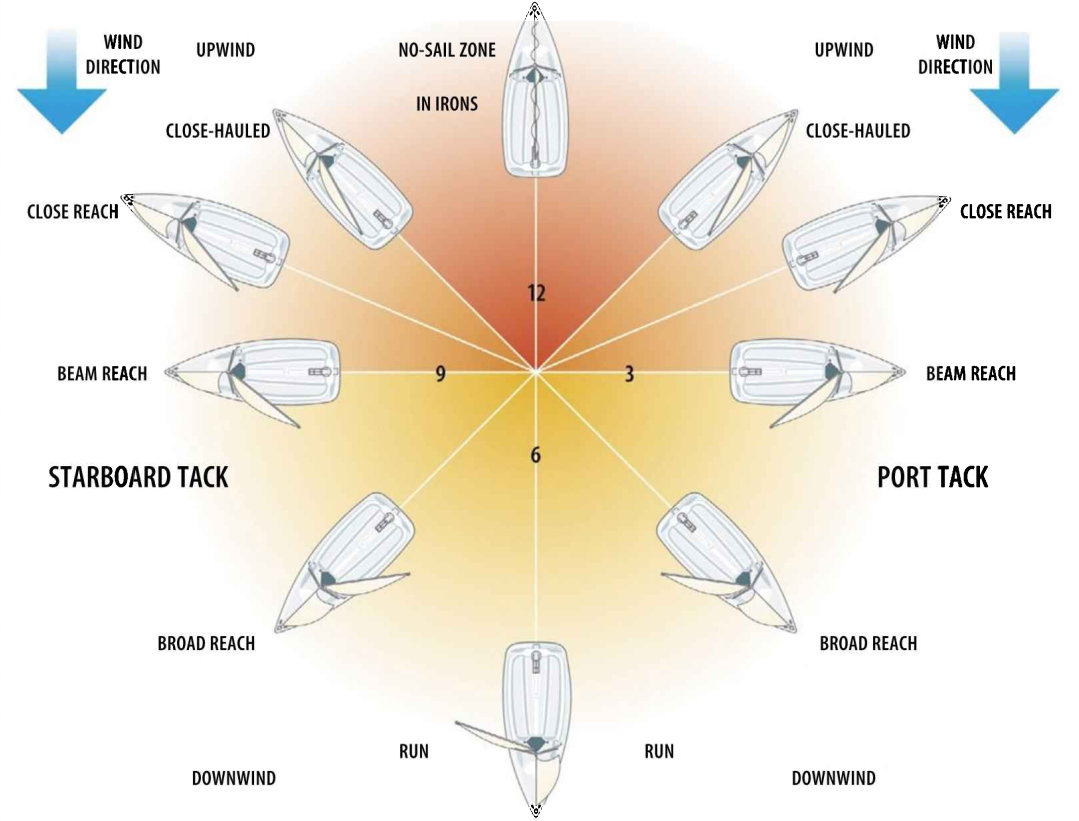
\includegraphics[width=0.7\linewidth]{point_of_sail.png}
    \caption[Point of sail]{Point of sail\cite{ASA} }
    \label{fig:point_of_sail}
\end{figure}

Point of sail is traditionally measured analogous to a clock, as shown in Fig. \ref{point_of_sail}. For the purpose of this report point of sail will be defined 
as the angle between apparent wind direction and the direction of travel of the boat, measured clockwise in degrees. A sail direction of $0^{\circ}$ will 
then correspond to 12'oclock in Fig.\ref{point_of_sail} and $180^{\circ}$ will corresponding to 6'oclock measured clockwise. The position of the mainsail will be 
defined by the angle between the mainsail and the centerline of the sailboat to either the starboard or port side.

If the desired destination is within the no-sail zone, a manoeuver known as 'tacking' can be performed to reach the desired destination. When sailing with 
he wind blowing on the starboard, its on the starboard tack, and when the wind is blowing on port side, the boat is on port tack. Tacking is the act of 
turning the bow of the sailboat through the no-sail zone. Assume the boat is on starboard tack and point of sail is $45^{\circ}$, after some distance has been travelled 
the bow is turned through the no-sail zone to attain a port tack and a point of sail of $-45^{\circ}$, this 'zig-zag' motion is done continuously until the 
desired destination is reached.

Another important manoeuver is the 'jibe', which is defined as the action of changing from a starboard tack to a port tack. An example of this occurring is when 
point of sail changes from $160^{\circ}$ to $100^{\circ}$, initially apparent wind will be port side but after crossing over $180^{\circ}$ the wind will be starboard side, 
during this crossover the mainsail will often swing from starboard to port.
\section{Related Work}

\subsection{Unmanned Sailing Vessel by Philip van Schalkwyk}
Philip is a mechatronics graduate who designed and developed an unmanned sailing vessel for his final year project at Stellenbosch University \cite{Phillip}.

\subsubsection{Objectives}
The purpose of the project was to design and develop an USV that is capable of semi-autonomous sailing. The objectives are as follows:

\begin{itemize}
    \item Design and develop a low-cost digital compass that produces accurate readings with tilt compensation.
    \item Design and develop a a low-cost mechanical wind vain that consists of a digital compass for wind direction sensing.
    \item Retrofit a RC sailing vessel with a micro-controller, digital compass, wind direction sensor, GPS unit and micro-SD card.
    \item Design and implement navigational and control systems to enable autonomous sailing.
\end{itemize}

\subsubsection{Method Used}
A RC sailing vessel was retrofitted with a micro-controller that would read data from sensors and adjust the rudder and sail position in order to sail along a 
desired path. The system consisted of a micro-controller, GPS receiver, a micro-SD card, an digital compass, wind direction sensor and two servo motors - one to control the 
sail and one to control the rudder angle. The micro-controller that was used was a Espress ESP-WROOM-32 micro-controller which is relatively low cost and has 
a 240 MHz clock speed. The electronic compass was used to determine the current bearing of the vessel, it was designed and developed using a magnetometer, 
accelerometer, gyroscope and tilt compensation algorithms. The MPU9250-6500 9-axis sensor module was used for the electronic compass as it consists of a magnetometer, accelerometer and a 
gyroscope. A mechanical wind vain was designed with CAD software and printed with a 3D printer. The wind vain
was fitted with a magnetometer - also the MPU9250-6500- which was used to determine the bearing of the wind vane and therefore the wind direction. The GPS receiver that was used for the navigational
system was a Neo M8N GPS, it would log positional data to the micro-SD card. 

A proportional controller was used to control the rudder position. The desired heading/bearing was calculated using the current GPS coordinates obtained from the 
GPS receiver and the target GPS coordinates. A sample would then be taken from the electronic compass which would give the current bearing of the vessel, the difference 
the current bearing and the desired bearing is the error signal. The proportional controller would then determine the rudder angle given this error signal, and the servo 
motor controlling the rudder would be adjusted accordingly. 

The main sail position was determined by the samples taken from the wind direction sensor and the current bearing. Only three point of sail classifications were used for the sail positions 
: close-hauled, beam-reach and run. This was done to give more time to navigational and rudder control systems. If it was determined that angle of attack was less than $45\deg$
the vessel would tack into the wind. This was achieved by calculating the bearing to either side of the no-sail zone, the vessel would then sail with one of these bearings for 50 meters 
and then change to the other bearing. The vessel would alternate along these bearings until the target destination was reached.

\subsubsection{Results}
The e-compass was tested against a magnetic compass and the results showed the average error in bearing to be $5.84^{\circ}$, the e-compass did however produce a consistent spike at $180^{\circ}$ across
multiple tests. Tests that were done with the GPS receiver showed that the positional accuracy of the GPS receiver was sufficient for the navigational system and data-logging. The wind sensor that
was developed was unable to provide wind direction data consistently, a possible explanation for this is that the length of the $I^{2}C$ connection is too long and therefore the capacitance in the lines caused 
a low pass filter effect on the signal. In the final tests that were conducted to verify the successful operation of the control systems, the point of sail classification was set to run initially and sail adjustments were not taken 
throughout the duration of the test - due to the wind sensor not working. The results of the final test showed that the rudder control system was capable of keeping the vessel on a near constant 
heading, with a maximum absolute error of $6\circ$. This test was conducted between two GPS coordinates and the vessel therefore sailed on a fixed bearing between them. Fig \ref{fig:phillip_lake_test} shows
the results of this final test.

\begin{figure}[!h]
    \centering
    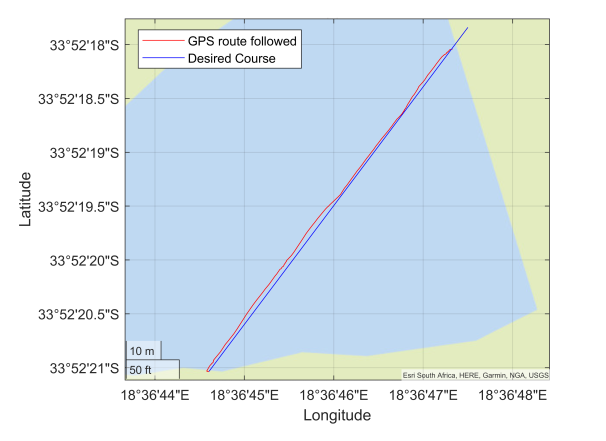
\includegraphics[width=0.918\linewidth]{phillip_lake_test}
    \caption[Test results from lake test]{Test results showing deviation of vessel from ideal trajectory \cite{Phillip}}
    \label{fig:phillip_lake_test}
\end{figure}

\subsubsection{Remaining challenges}
The rudder control system designed by Phillip was capable of accurately tracking a desired bearing during tests. Proportional integral control could not be implemented due to the consistent error that occurred during 
the e-compass testing. The USV that was developed does not however have the ability to dynamically adjust the sail position according to the relative wind direction, and is therefore unable to achieve the desired 
performance if wind direction is not constant. Tests where also not conducted to verify the tacking capabilities of USV.

\subsection{Design and Implementation of a Control System for a
Sailboat Robot}
\label{sec:robotics-paper}

\subsubsection{Objectives}
\begin{itemize}
    \item Determine the dynamic equations that govern the behavior of a sailboat.
    \item Use the dynamic equations to design - through simulation- a simple, however effective, controller that can be applied to different types of sail boats.
    \item Develop a prototype sailboat to implement and test a controller which was designed through simulation.
\end{itemize}

\subsubsection{Method Used}

The system that is developed for an autonomous sailboat consists of two processing units, a combination of sensors, and actuators/servos. Two processing units are used for a more 
flexible system. The one processing unit is a ATMega2560 which is built into an arduino, and is used to handle low level control decisions that should be executed in real time. 
The arduino communicates with the various sensors and implements the control algorithms used to control the actuators in a stable manner. The other processing unit is a Raspberry 
Pi which is responsible for high level navigation decisions, planning and external communication. The Raspberry Pi is connected to a base station via a XBee radio link of up to 1.6 Km. 
The two two processors communicate with each other via a RS-232 serial connection. The sensors that are used consist of a GPS receiver (EM-406 SiRF III), and a three axis digital compass 
(actual component used is not specified). A wind sock is used to determine wind direction and this is then transmitted to the system from the base station via XBee. Digital compass
is calibrated to compensate for local magnetic declination. 

The approach used to design an appropriate control system for an autonomous sailboat is to mathematically model the dynamics of the sailboat, and then through simulation, identify 
the optimal parameter values of the controller. Determining the dynamics that govern the behavior of a sailboat are divided into calculations of hydrodynamics, moment of inertia, 
viscous damping, lift, effort sail and centre of mass. These calculations are combined to form Eq. \ref{eq:sail_dynamics} which is used as the control law that governs sailboat control. 
In Eq. \ref{eq:sail_dynamics} $M_{a}$ refers to the hydrodynamics, $C_{rb}$ is dynamics(including centre of mass), $C_{a}$ refers to hydrodynamics related to coriolis and centripetal forces, 
$D_{k}$ term is the lift moments generated by the keel and $D_{h}$ are the lift forces acting on the hull.

\begin{equation}
    ( M_{RB} + M_{A} ) \dot{\upsilon} = \tau_{s} + \tau_{r} - (C_{RB}(\upsilon) + C_{A}(\upsilon))\upsilon  - (D_{k}(\upsilon) + D_{h}(V))V - g(\eta)
    \label{eq:sail_dynamics}
\end{equation}

Two controllers are initially developed: a PID controller for rudder control, and a fuzzy controller, which controls the sail position. By making use of Eq. \ref{eq:sail_dynamics} and simulation 
software (MATLAB) optimal parameter values are found for the PID controller. This approach is faster than the traditional method of adjusting the parameters, however since the 
mathematically model does not truly represent the sailboat the parameter values found are used as initial values to be further adjusted through experimentation.

The rudder controller takes in an error signal as its input and outputs the appropriate control signal to the rudder actuator. The error signal is determined as the difference 
between the actual bearing of the sail vessel and the desired bearing of the sail vessel. Desired bearing is calculated using current GPS location of the vessel and the target 
GPS location. The actual bearing of the sail boat is determined from the digital compass. 

The sail controller takes wind direction as its input and adjusts the sail position accordingly, the controller also takes into account limits of the sail vessel i.e. the dead-zone/no-sail zone.

In the sailboat prototype that is developed, the D parameter used in rudder control is disregarded, mainly because of instability, which is generated due to intensification 
of high-frequency noise caused by the derivative. 

\subsubsection{Results}

In the simulation the optimal gains for the rudder controller are: Kp = 0.68, Ki = 1.125 and Kd = − 0.130. These controller gains were used as initial values to be fine-tuned through
multiple tests done with the prototype sailboat. After conducting the tests the resulting adjusted rudder controller gains were: kp = 2.3 and ki = 0.8. The tests that were done 
compared the use of a proportional controller and a PI controller for the rudder control, Fig.\ref{fig:robotics_test_result} shows the results of one of the tests. Note that the 
sailboat was initially placed to face $90^{\circ}$ from target location. In all tests that were conducted the prototype sailboat reached the specified target coordinates, the PI 
controller, however, performed better than the P controller with less deviation from the ideal trajectory.

\begin{figure}[!h]
    \centering
    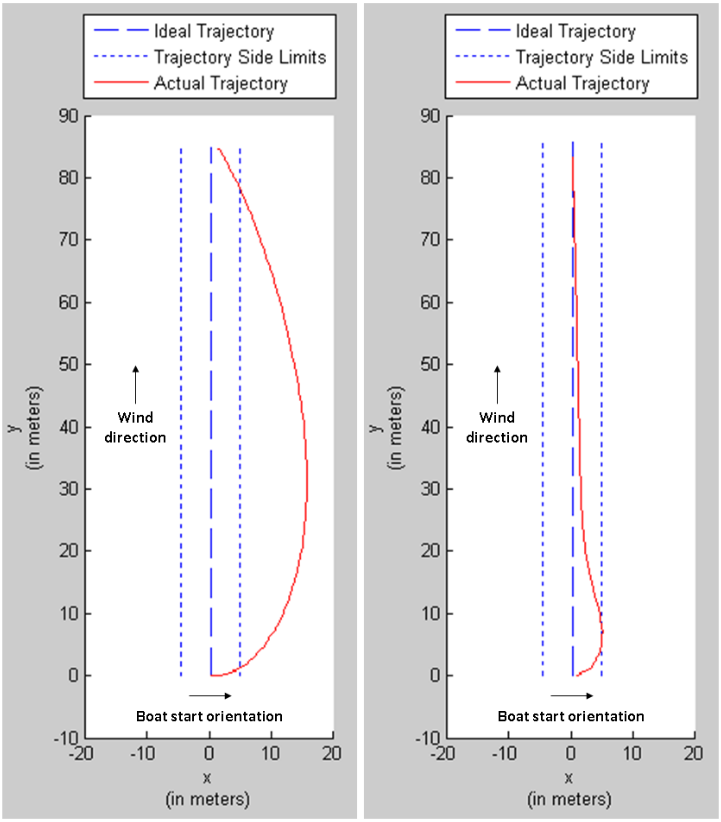
\includegraphics[width=0.6\linewidth]{robotics_test_result}
    \caption[Test results comparing P controller and PI controller]{Test results on water; P controller shown left and PI controller on right \cite{robotics5010005}}
    \label{fig:robotics_test_result}
\end{figure}

\subsubsection{Remaining challenges}

The system that was designed and developed does not incorporate an onboard wind direction sensor but instead receives the wind direction data from a base station via XBee. 
The sail vessel will therefore not be capable of travelling distances over which the apparent wind direction around the vessel differs from the wind direction around the base 
station. Aside from this, the system that was developed addresses the problem statement in section \ref{problem_statement}; the purpose of the following sections is then to duplicate the 
above system.


\subsection{FASt - An autonomous sailing platform for oceanographic missions}
the purpose of this project was to design and develope an autonomous sailing boat to enter the Microtransat competition - competition for fully autonomous sailing boats wherein the goal 
is to cross the atlantic ocean \cite{Alves2008FAStA}.

\subsubsection{Objectives}
\begin{itemize}
    \item Design and construct a high performance and light-weight sailboat of suitable size.
    \item Design and develope an electronics system that will enable long distance autonomous navigation and control of the sailboat.
    \item The electronics system must include a communication subsystem for short range and long range communication.
    \item The electronics system should have a low power consumption and powered by a power source that is recharged via photovoltaic cells.
\end{itemize}

\subsubsection{Method Used}
The sailboat hull shape was inspired by modern racing oceanic yachts and was constructed with fiber glass and epoxy resin. The total length of the sailboat is 2.5 m with a mast height 
of 3.4 m. It features two independently controlled rudders and two sails which are controlled simultaneously

The electronics system was divided into 5 subsystems: computing, communication, sensors, actuators and power management. The computing system consists of a 32-bit RISC microprocessor 
running with a maximum clock speed of 50 MHz, ROM memory which holds the bootstrap code and various digital modules that interface the processor with the sensors and actuators. The 
computing system was implemented using a FPGA, the one that was used was a Suzaki SZ130 which is built around a Xilinx FPGA. The board includes central Microblaze processor running
at 50 Mhz, 32 MB of SDRAM, 8 MB of SPI flash memory, a serial interface (RS232) and ethernet port implemented externally to the FPGA. The board has 86 input/output pins available,
which connect directly to the FPGA. The computing system runs uCLinux which a version of linux which has been simplified and adapted for embedded applications running processors 
with no memory management unit. The advantage of using an FPGA is that many of the processing and interfacing functions of the system can be implemented in custom hardware and 
therefore are not managed by a micro-processor; this allows the use of a micro-processor that runs at significantly lower clock speeds and thus lower overall power consumption.

The communications subsystem consists of a conventional WiFi router (LinkSys WRT54GC), a GSM modem (Siemens MC35), a IRIDIUM SBD modem (model 9601) and a radio control receiver. 
The WiFi router is to provide convenient short range communication with a laptop, mainly for the purpose of software development, debug and communication purposes. While at sea 
missions, the GSM modem and IRIDIUM SBD modem will enable small volume communications to take place. The GSM module enables communications within a range of a few kilometers from 
shore, the IRIDIUM SBD modem communicates via satellite connection and allows and therefore has a global range. The radio control receiver allows for manual control over the sailboat
 using a 4 channel proportional control RC transmitter.

Sensors used consist of a wind vane, anemometer, boom position sensor, digital compass (LinkSys WRT54GC), GPS receiver(uBlox RCB-4H), inclinometer, voltage monitors, ambient light 
sensor, interior temperature and a set of water sensors. The wind vain and boom position sensors were custom built using a magnetometer (Austria Micro Systems AS5040) and are used 
in the sail position control system. The anemometer is a conventional cup rotor that makes use of a hall effect switch, its main purpose is for data collection and data logging during 
sea missions. The digital compass and the GPS receiver are used for navigation and data logging purposes. The inclinometer is used to determine heel angle which is used to reef the sails. 
It should be noted that the sailboat that was developed does not have the ability to adjust the area of the sail i.e. reef, the inclinometer was included for future iterations of the 
project that possess have this ability. The voltage monitors are used to monitor the voltage of the batteries. The ambient light sensor is used to monitor light intensity which affects
 the voltage produces by photovoltaic cells. Specific hardware was designed and implemented in the FPGA to interface these sensors with the RISC micro-processor.

The actuators in the system consist of two standard high-power RC servos which provide independent control of the two rudders. The two sails are both controlled simultaneously by a 
DC geared motor. Although having a low efficiency the DC geared motor is extremely robust, and once position and un-powered the gearbox locks the motors shaft in place. Traditional 
servo motors consume power in holding a certain shaft position in response to an applied force on the shaft. The use of the DC geared motor is therefore advantageous as sail position
is only adjusted when changing course or if a change in wind direction occurs, therefore no power is consumed in keeping the shaft fixed in reaction to the force applied by the wind. 
A multiplexer was implemented in hardware to select the source data that is routed to the actuators, if a RC connection is established then this data is selected, otherwise data from 
the computing system is selected.
 
The power management system consists of a 45 Wp solar panel (Solara SM160M), two 95 Wh Li-ion batteries, a battery charging circuit and a highly efficient power supply. A wind generator
was considered to compliment the photovoltaic cells but ones available commercially are too large and heavy for this application. The total power consumption of the system was measured
to be 560 ma.

The software is divided into five modules that implement the five main tasks: hardware interface, helm, sail, skipper and logger. The hardware interface implements all the driver 
software needed for the processor to communicate with sensors,actuators and configuration parameters. The helm implements the PI controller used to control the rudder position according
 to wind direction and desired bearing. The commands supported by this module include keeping a fixed bearing, maintaining the angle of apparent wind and performing tacking or gibing 
 maneuvers. The sail module is responsible for controlling the sail position according to wind speed and direction and a set of rules that define best sail angle. This module also implements 
 reefing of the sails - the sheet is eased when heel angle is greater that a certain value. The skipper module sends commands to the helm and sail modules and is responsible for higher
  level navigation such as deciding what course to follow and when to perform certain sailing maneuvers. The logger module listens to all the other modules and stores relevant data in a log file.

\subsubsection{Results}
This article does not cover the testing of the system described above and therefore the validity of the design cannot be verified. The article does however highlight important hardware 
and software design features to consider when attempting to design an autonomous sailing vessel

\subsubsection{Remaining challenges}

The system made use of an FPGA to implement the central computing system as well as interface with the sensors and actuators of the system. While this
 does decrease the power consumption of the system it also greatly increases the complexity of the design. Many modern micro-controllers already incorporate the hardware needed to 
 interface with the various sensors and actuators used in this system. 

Given that the scope of this project stated in section \ref{}, low power consumption of the system, although important in long distance sea missions, is not of vital importance for 
the purpose of designing and developing the navigational and control systems for an autonomous sail vessel. 

The system included functionality that is not needed for the purpose of this project. Some of this functionality includes the simultaneous 
control of two sails, two rudder servo's, boom position sensing, wind speed sensing, heel angle sensing, a power supply that incorporates rechargeability and photovoltaic cells, and a 
communications subsystem for short and long range communication with the vessel.

\subsection{Establishing frame of reference}
\label{sec:reference_frame}

It is important to establish a fixed frame of reference which can be used to determine the orientation of a vessel at sea. The fixed frame of reference that will be used in this report 
is the industry standard "NED" (North, East, Down) coordinate system. The NED coordinate system is orientated such that at any position on the earth the x-axis is aligned with true north, 
the y-axis is aligned with lines of latitude and points east, the z-axis is aligned with the vector that represents the acceleration of gravity. The x,y-plane is therefore tangent to the 
sphere of the earth. The inertial frame of the sailing vessel is fixed to the body of the sailing vessel and is the perspective that a person on the sailing vessel would have. The x-axis of 
the inertial frame of the sailing vessel is aligned with the centerline of the vessel and points from the stern to the bow, the y-axis is aligned perpendicular to the centerline of the vessel
and points to the starboard side, the z-axis is aligned with the mast of the vessel and points downwards. This concept is illustrated in Fig. \ref{fig:reference_frame}. 

\begin{figure}[!h]
    \centering
    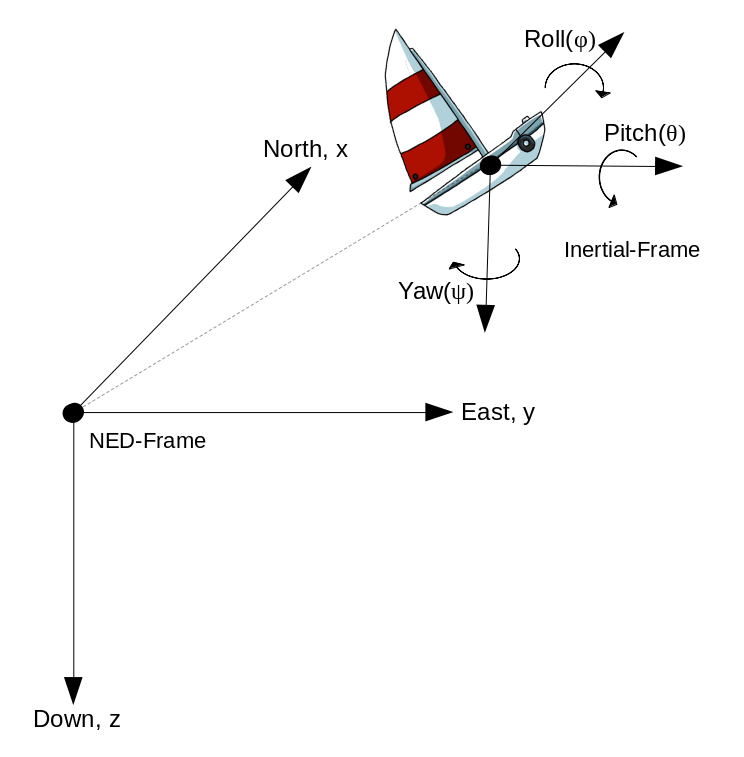
\includegraphics[width=0.5\linewidth]{reference-frame.png}
    \caption[NED frame of reference]{NED frame of reference}
    \label{fig:reference_frame}
\end{figure}

Rotation of the inertial frame about the x-axis is known as the roll angle ($\phi$), rotation about the y-axis is the pitch angle ($\theta$), and rotation about the z-axis is the yaw angle 
($\psi$). For all axes, clockwise rotation is taken to be positive rotation. Given that the roll, pitch, and yaw angles are all known it is possible to transform the inertial frame back to 
the NED frame using transformation matrices in Eq. \ref{eq:R_x}, \ref{eq:R_y}, \ref{eq:R_z} \cite{e_compass}. 

\begin{equation}
    \vec{R_{x,\phi}} = \begin{bmatrix} 1 & 0 & 0 \\ 0 & \cos\phi & -\sin\phi \\ 0 & \sin\phi & \cos\phi \end{bmatrix}
    \label{eq:R_x}
\end{equation}

\begin{equation}
    \vec{R_{y,\theta}} = \begin{bmatrix} \cos\theta & 0 & \sin\theta \\ 0 & 1 & 0 \\ -\sin\theta & 0 & \cos\theta \end{bmatrix}
    \label{eq:R_y}
\end{equation}

\begin{equation}
    \vec{R_{z,\psi}} = \begin{bmatrix} \cos\psi & -\sin\psi & 0 \\ \sin\psi & \cos\psi & 0 \\ 0 & 0 & 1 \end{bmatrix}
    \label{eq:R_z}
\end{equation}

\subsection{Magnetic declination}

A traditional handheld magnetic compass will align itself with the earths local magnetic field lines, which in theory run from the magnetic south pole to the magnetic north pole. This 
means that a magnetic compass will point to magnetic north. However in practice this is not true, the earths magnetic field lines are not constant, and depending on where measurements
are taken there will exist an angle of error. True north is defined as  

True north, also known as geographical north, is defined as the point where all lines of longitude intersect. Magnetic north is the point to which a magnetic compass aligns itself, and 
varies across the globe as well as with time. The direction of magnetic north differs depending location because earths magnetic field lines do not travel a linear path from magnetic 
south to magnetic north, this is illustrated in Fig. \ref{mag_declination}. 

\begin{figure}[!h]
    \centering
    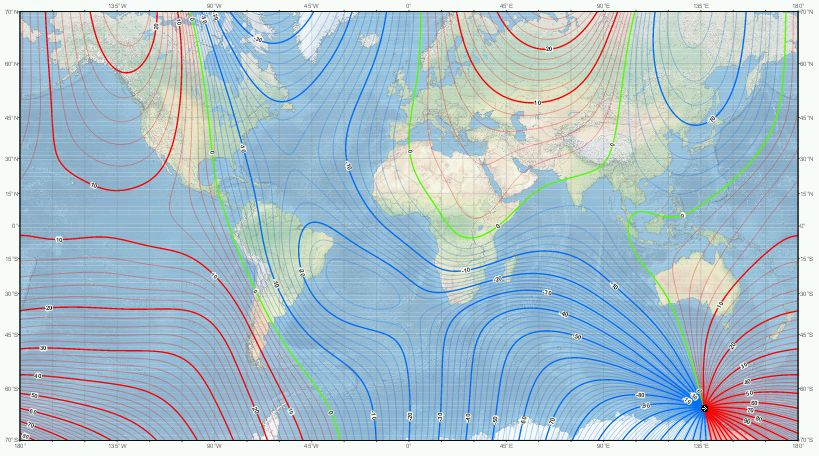
\includegraphics[width=0.9\linewidth]{mag_declination}
    \caption[Magnetic declination across the globe]{Magnetic declination across the globe \cite{Mag_declination}}
    \label{fig:mag_declination}
\end{figure}


Magnetic declination is an angle of correction used to determine true north from a local magnetic north reading. Magnetic declination takes into account the variance of local magnetic 
field lines and the angle between magnetic north and true north. Magnetic declination therefore differs across the globe. The National Oceanic and Atmospheric Administration (NOAA) \
keeps track of magnetic declination across the globe as it changes with time. The magnetic declination in Stellenbosch is $25.77^{\circ} \pm 0.59^{\circ}$.   
\graphicspath{{system_design/fig/}}

\chapter{System Design}
\label{chap:system_design}

\begin{figure}[!h]
  \centering
  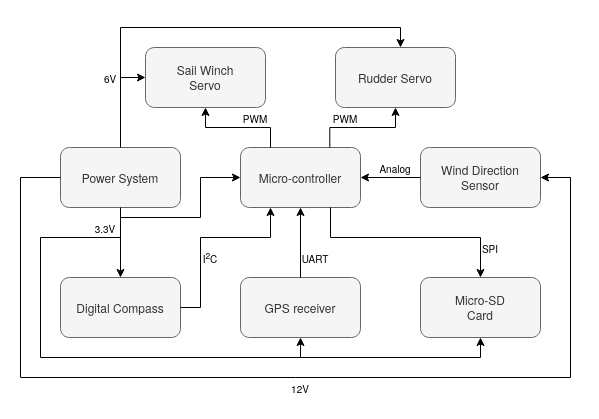
\includegraphics[width=0.918\linewidth]{system_diagram.png}
  \caption[System Diagram]{System Diagram}
  \label{fig:system_diagram}
\end{figure}

\section{Sail Vessel}
The sailing vessel houses the entire system illustrated in Fig. \ref{fig:system_diagram}. Designing and developing a sailboat is a complex task on its own, 
requiring expertise and experience in many fields, some of which include aerodynamics, hydrodynamics and material design. Given the complexity of this task 
and the time constraints of the project, an existing RC sailboat was used. A Dragonflite 95 RC sailboat\cite{Dragonflite} was modified to incorporate the system illustrated 
in Fig. \ref{fig:system_diagram}. The Dragonflite is 950 mm in length and has an overall weight of two kilograms. It features two sails (mainsail and jib),  
a carbon fibre mast and moulded carbon fibre keel with zinc alloy ballast bulb. The sailboat is operated
with a 2.4Ghz 4-channel digital proportional transmitter which communicates with a 2.4Ghz 4-channel receiver. The Dragonflite 95 comes preinstalled with a rudder 
servo motor as well as a sail winch servo motor. The sail winch servo controls both the mainsail 
and the jib simultaneously. The receiver and two servo motors are powered with a 6v battery source (4 AA batteries). The transmitter and receiver were 
removed as they are not needed in the development of a autonomous sailboat.

\section{Micro-controller}
Two options were considered for the micro-controller: the Adafruit BlackPill STM32F411 development board \cite{black_pill} and a Adafruit STM32F405 Feather \cite{STM32F405-specs}.
 The Adafruit BlackPill
has an Arm 32-bit Cortex-M4 CPU, which has a clock speed of 100MHz, 512KB flash memory, 128kB SRAM, and has a power efficiency
of $100\mu A$/$MHz$. The Adafruit feather has an Arm 32-bit Cortex-M4 CPU, with a clock speed of 168 MHz, 1MB flash memory, 
and has a power efficiency of $238\mu A$/$MHz$. Despite the higher price and power consumption of the Adafruit Feather, it was chosen for this system as it has a 
higher clock speed, which is needed for the navigational and control systems. The Adafruit feather also has a jst connection for a lithium-polymer battery as well as a 
3.3V regulator.


\section{Wind direction sensor}
The direction of apparent wind is needed to determine the optimal positioning of the sails. Wind direction sensors that were considered where: an ultrasonic 
anemometer, a mechanical wind vain, and the development of a wind direction sensor using four electret microphones and correlating the signals. The ultrasonic
anemometer that was considered was the WS303U by Sentec Meteorology, it was not used because it is too large for the sailing vessel. The development of a 
wind direction was not done because of the time constraints of the project. The mechanical wind vain was chosen as the most viable option. The sensor used was 
the FST200-202\cite{wind_sensor} made by firstrate sensor company. This sensor is designed for outdoor environments such as weather stations and boats, it therefore has 
excellent resistance to extreme weather conditions and erosion. The sensor works in wind speeds greater than 0.8 m/s, has a $22.5^{\circ}$ resolution and 
$\pm 3^{\circ}$ accuracy. It features automatic temperature compensation and operates in a temperature range of $-20^{\circ}C$ to $+85^{\circ}C$. The 
sensor has a working voltage of 12~30VDC, and its output is a 4-20 mA signal. 

\section{Servo motors}
Two servo motors are required: one for controlling the mainsail, and the other for controlling the rudder. The decision was made to use the preinstalled servo motors as 
the vessel was designed operate with these specific 
servo motors, it also keeps system design costs low. The manual specifies that a metal geared servo is used for rudder control
and a sail winch servo is used to control the sail position. Aside from this, no other information is given in the manual about the servo motors.  

\section{GPS receiver}
The GPS receiver is used to determine the GPS coordinates and speed of the sailing vessel. GPS coordinates of the vessel are needed to calculate the reference bearing 
(used in rudder control),
which is the bearing between current position and the target position. All GPS receivers on the market are accurate to within 2.5m, component choice is 
therefore dependant on factors such as price, power consumption and update rate.The GPS receiver that is used is a ATGM336H-5N\cite{GPS} module. It was chosen because it 
has a high tracking sensitivity, low power consumption and is low cost. Supply voltage of the receiver is 3.3V and it communicates via a UART interface. It has a 
tracking sensitivity of -162dBm, consumes $<25mA$ during continuous operation, 
has a first positioning time of 32 seconds, maximum update rate of 10Hz, and also features built in antenna short circuit protection.

\section{Digital compass}
The digital compass is used to determine the bearing of the sailing vessel, which is compared to the reference bearing to determine if the vessel is off course. It is 
required that the compass be able to perform tilt compensation, as the vessel will not always be on a level surface out at sea. The error in heading that occurs when tilt
compensation has not been implemented is illustrated in Fig.\ref{fig:tilt_error}, where it can be seen that as the pitch angle of the vessel increases, a greater error in 
heading occurs\cite{tilt_error}. To perform tilt compensation a magnetometer is needed to determine magnetic field vector, and a 
accelerometer is needed to determine the acceleration due to gravity vector. An IMU is a device that contains both a 3-axis magnetometer, 3-axis accelerometer and 3-axis gyroscope.
The two options that were considered were a AltIMU-10-V4\cite{altimu-10} made by Pololu Electronics and a MPU-9250/6500 9-axis IMU\cite{mpu-9250}. Both options feature 
16-bit ADC with signal conditioning. The 
Alt-IMU-10-V4 also features a digital barometer which is not needed for the purposes of this project. The MPU-9250/6500 was chosen for its low cost when compared 
to the AltIMU-10-V4. The MPU-9250/6500 has a supply voltage of 3.3V, an operating current of 3.5mA and an $I^{2}C$ interface.

\begin{figure}[!h]
  \centering
  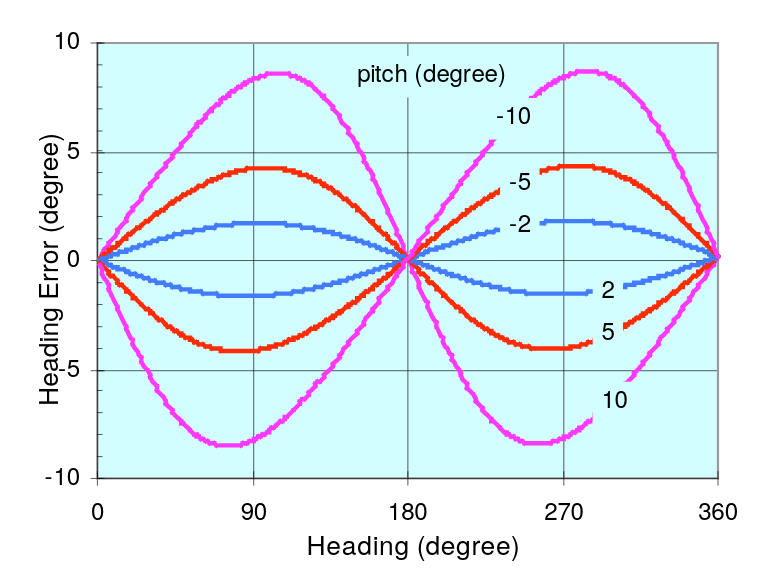
\includegraphics[width=0.5\linewidth]{tilt_error.png}
  \caption[Tilt error]{Heading error due to tilt without tilt compensation\cite{tilt_error}}
  \label{fig:tilt_error}
\end{figure}


\section{Micro-SD card}
The Micro-SD card is used for data-logging purposes, it allows for data from tests to be stored and analysed at a later time. Data that is logged during water tests 
include: current position, current bearing, desired bearing, bearing error, distance to target, wind direction, and tracking speed. A micro-Sd card socket made 
by Pololu\cite{sd} was used, and features a SPI.  


\section{Power system}
The power system consists of three separate power sources. The rudder servo and sail winch servo are powered by a 6v battery source consisting of four 1.5V
alkaline batteries in series. The Adafruit feather is powered by a 5000mAh 3.7V lithium polymer battery. The Adafruit feather is used to power the micro-SD 
card socket, GPS receiver, and digital compass. The wind direction sensor is powered with two 9V alkaline batteries in series. The use of one 12V power source 
with a 3.3V regulator was initially considered. Three separate power sources were chosen because the power consumption of the system is such that two 9V alkaline
batteries would only power the system for 2.13 hours, which was considered insufficient.
 %Discuss reason you used three
%different power sources instead of one. could say low cost?

\section{Metrics}


% \item Design and develop a digital compass that compensates for tilt.
% \item Determine and compare the accuracy of bearing obtained from a GPS receiver and that from a digital compass.
% \item System must be capable of logging operational data to a micro-SD card.
% \item Design and implement necessary navigational algorithms: Determine distance and bearing between two GPS coordinate.
% \item Design and develop sail control system.
% \item Design and develop rudder control system.
% \item Design and implement tacking manuever into system.

\subsubsection{Data logging}
To verify the system is capable of logging data as well as test the successful operation of the GPS receiver, a simple test is conducted. The experimental 
setup is as follows: The system is carried along a path, the GPS receiver will take samples at a rate of 1Hz, the GPS coordinates will then be logged to 
the micro-SD card on each sample, results are then analyzed to determine if path that was logged corresponds to the actual path travelled. 

\subsubsection{Digital compass}
Successful operation and accuracy of the digital compass is determined with two separate tests. 

The first test is done to test the accuracy of the digital 
compass. The setup is as follows: the digital compass undergoes extensive calibration; the digital compass as well as a handheld magnetic compass shown 
in Fig. \ref{}, are placed on a level piece of wood and 
spaced such that they do not interfere with each other; the wood is rotated in steps of $10^{\circ}$ anti-clockwise; each step readings from the handheld 
compass and the digital compass are taken and compared; because of the slight sample deviation present in the digital compass, an average of 10 samples
are taken for each step. 

The second test is done to determine the successful operation of the tilt compensation algorithm that is used. The 
setup is the same as the first test, but this time a pitch angle of $10^{\circ}$ is applied to the digital compass, the handheld compass is still placed 
flat. Again the wood is rotated in steps of $10^{\circ}$ anti-clockwise, and again ten samples are taken from the digital compass on each step, the average
of these samples is used for comparison. The results of this test are compared with the results from the first test - where the digital compass had a pitch 
and roll angle of zero. 

Accuracy of the digital compass needs to be compared with that of the GPS receiver. If the GPS receiver is capable of determining the bearing with better/or 
even the same degree of accuracy as that of the digital compass, then the use of a digital compass in the 
system does not make sense. It should be noted that the GPS receiver is only capable of determining bearing when the velocity of the system is greater than
zero. The test done to compare the accuracy of these two components is as follows: The GPS receiver is carried along a path of constant bearing and with a 
velocity similar to that of the maximum velocity the sailboat is capable of, bearing samples are then taken at a frequency of 1Hz, the same is then done 
for the digital compass, digital compass is held such that it points to the end point of the path throughout 
the test. The digital compass must be calibrated before the test. The results of the two tests are then compared.  

\subsubsection{Navigational calculations}
The successful operation of the algorithm used to determine distance between two points is verified using the following experimental setup: a target GPS 
coordinate is given to the system, the current GPS coordinates are obtained from the GPS receiver at varying distances from the target and distance is 
calculated, distances that samples are taken are physically measured out before the test is done, an average of ten distance calculations are done for each
change in distance. 

% Should include test to verify bearing here?

\subsubsection{Sail control}
A test will be conducted to verify accuracy as well as successful operation of the sail control system. The experimental setup is as follows: wind direction 
sensor will be adjusted in $22.5^{\circ}$ increments - wind sensor's resolution - with $0^{\circ}$ corresponding to center on no sail-zone, corresponding 
change in sail position will then be measured from the centerline of the boat.

\subsubsection{Rudder control}
The first test will test the operation of the rudder control out of the water. A target GPS coordinate will be chosen and given to the system, the system 
will then be carried along a path of constant bearing ending in the target coordinate, the current position, desired bearing, actual bearing and error signal
will be logged throughout the test. 

The second test will be done on the dam by the Maties canoe club. The experimental setup is as follows: a target coordinate is programmed into the system,
the digital compass is calibrated and the sailboat is placed at a suitable starting location. Apparent wind is determined beforehand and the sail position is 
set accordingly (sail position control will be disabled for this test). The data that will be logged throughout the test is: current GPS coordinate, distance 
to target, desired heading, actual heading, heading error signal, rudder PWM value and apparent wind direction. The purpose of this test is to evaluate the performance
of the rudder controller and determine optimal gains through experimentation, this test will therefore be repeated more than once.

\subsubsection{Sytem}
A similar test will be done on water at the Maties canoe club to verify the successful operation of the entire system - navigational and control systems. The test
is similar to the second test done for the rudder control except the sail control will be included, and the setup is as follows: a target coordinate is 
programmed into the system and the digital compass is calibrated, the sailboat is placed at a suitable starting point, data will be logged throughout the test. 
The data that is logged is: current GPS coordinate, distance to target, desired bearing, actual bearing, bearing error signal, rudder servo PWM value, apparent 
wind direction, sail position value, sail servo PWM value.

The final test will have the same experimental setup as the previous test, only difference being that two separate waypoints will be set beforehand. This test is 
done to verify the vessels ability to navigate to a single waypoint and then change navigation to a different waypoint. 







\graphicspath{{detail_design/fig/}}

\chapter{Detail Designs}
\label{chap:detail_design}

\section{Micro-controller}
% discuss how all functional blocks connect and communicate with each other 
The Adafruit STM32F405 feather has a supply voltage of 3.7V and consumes up to $80mA$ when operational, it is powered by a 5000mAh 3.7V lithium polymer 
battery connected with a jst connection. The board features a 3.3V regulator which is to regulate the battery power, there are also pins to distribute 
the 3.3V regulated power off-board. The 3.3V regulator is used to power the GPS receiver, MPU-9250/6500 IMU, and the micro-SD socket. The board has a USB-C 
female connector which is used to load the main program and for debugging during the design process. The board is capable of running circuit python, which was
used in the development of this project. 
%Not sure if i should mention this :(


\section{GPS receiver}
The GPS receiver has a power supply voltage of 3.3V and is powered by the Feathers 3.3V regulator. It is connected to a pin on the feather which is 
configured as UART, with a BAUD rate of 9600. The GPS receiver continually receives data at a frequency which is set during the configuration process, in 
this case its every second. Data sent by the GPS receiver is in the form of ASCII encoded sentences which follow the NMEA protocol\cite{nmea}. The NMEA 
protocol defines a number of ASCII identifiers which occur at the beginning of each ASCII sentence, they are used to identify the type of data 
contained in the sentence. Table \ref{table:NMEA} shows the specific NMEA sentences which are relevant to this project and their corresponding ASCII 
identifiers.
\\

\begin{table}[!h]
    \centering
    \caption{NMEA sentence information}
    \label{table:NMEA}
    \begin{tabular}{ | m{10em} | m{25em} | }
        
        \hline
        \textbf{Sentence identifier} & \textbf{Description} \\
        \hline
        \$GPGGA & Global Positioning System Fix Data (Time, Latitude, Longitude) \\
        \hline
        \$GPGLL & Geographic Position, Latitude / Longitude and time. \\
        \hline
        \$GPGSV & GPS Satellites in view \\
        \hline
        \$GPVTG & Track Made Good and Ground Speed. \\
        \hline
        \$GPRMC & Recommended minimum specific GPS/Transit data (Latitude, Longitude, Speed over ground in knots, Track angle made true, Magnetic variation) \\
        \hline
    \end{tabular}
\end{table}

% Not sure it uses PMTK
% The GPS receiver can be configured by sending the appropriate PMTK command packets\cite{pmtk}. These commands are the same for all GPS receivers. The GPS receiver was
% set to send GGA and RMC NMEA sentences, and the update rate was set to $2Hz$ by sending the appropriate PMTK commands.

\section{Wind Direction Sensor}
The wind direction sensor has a supply voltage in the range 12~30VDC, and is powered by two 9V alkaline batteries in series. It is mounted on the bow of the vessel.
It outputs a $4-20mA$ analog signal,
which is connected directly to pin A4 of the Feather. Pin A4 on the Feather connects to a 5V tolerant pin on the STM32F405 micro-controller. This pin was 
configured to use one of the micro-controllers 12-bit ADC, which has a sampling range of $0V$ to $3.3V$. A shunt resistor with a value of $160\Omega$ is 
connected to the sensor output. This value was calculated to produce a voltage over the resister in the range of $642mV$ to $3.2V$. The Actual voltage range
measured over the shunt resister was $642mV$ to $3.07V$.

All pins on the STM32F405 micro-controller are capable of sinking or sourcing $25mA$ maximum, there is therefore no chance of the sensor damaging the micro-controller
pin. A digital buffer was initially considered to prevent the micro-controller from loading the sensor output circuit, but was not used as the ADC inputs are
high impedance. The STM32F405 data sheet\cite{STM32F405-datasheet} specifies that for an ADC input, the max external impedance allowed for an error below $1/4$ of the LSB is $50K\Omega$. 
The shunt resistors value is multitudes smaller than this.     

\section{Servo Motors}
Both the rudder servo motor and the sail servo winch are powered by a 6V source consisting of four 1.5V alkaline batteries. The rudder servo motor is connected to pin
A2 of the feather, the Sail winch servo motor is connected to pin D9 of the Feather. Both these pins are configured to output a 50HZ PWM signal, with a duty cycle set
by the rudder and sail position controllers. The rudder angle is measured from the centre line of the boat, this corresponds to the neutral position of the rudder. Positive 
rudder angle is measured from neutral position to the starboard side of the vessel, negative rudder angle is measured from the neutral position to port side of the vessel. 
Sail position is measured in degrees from the centre line of the vessel to either the port or starboard side. The maximum and minimum PWM values for both servo motors was 
determined experimentally and is summarized in table \ref{table:pwm}, along with the corresponding angles. Note that the sail position minimum angle is $10^{\circ}$, this 
is in accordance with the recommendations outlined in the sailboats manual.

\begin{table}[!h]
    \centering
    \caption{Servo motor PWM limits}
    \label{table:pwm}
    \begin{tabularx}{\columnwidth}{ | X | X | X | X | X | }
        
        \hline
        Servo motor & PWM\_Min & PWM\_Min corresponding angle & PWM\_Max & PWM\_Max corresponding angle \\
        \hline
        Rudder & 48 & $60^{\circ}$ & 102 & $-60^{\circ}$ \\
        \hline
        Sail & 75 &  $10^{\circ}$ & 120 & $80^{\circ}$ \\
        \hline
    \end{tabularx}
\end{table}

\section{Micro-SD card}
The micro-SD card socket has a supply voltage of 3.3V and is powered with the Feathers 3.3V regulator. It is connected to the Feather using a SPI interface. The micro-SD card sockets MOSI, MISO,
 and clock lines are connected directly to the corresponding pins on the Feather, the chip select line is connected to pin 6 of the Feather. The micro-SD card is formatted with the FAT32 file 
 system, and as, such writing to the micro-SD card is done with FAT32 protocol.


\section{Digital compass}
The MPU-9250/6500 IMUhas a supply voltage of 3.3V and is powered by the Feather boards 3.3V regulator. It is connected to the Feather via a $I^{2}C$ connection. The IMU has an address pin 
which is grounded. The purpose of the address pin is for setting the LSB of the $I^{2}C$, this allows two IMU's to be connected to the same bus, which is not needed in this case. 

\subsection{Tilt Compensation}

To perform tilt compensation, firstly pitch and roll angles of the inertial frame of the vessel must be found. Eq. \ref{eq:acc_1} is used to transform a sampled acceleration vector back to 
the NED frame of reference, where there exists only a z-component with magnitude 9.81 $m/s^2$. In this eqution $\vec{A}_s$ represents the acceleration vector which has been 
sampled from the IMU, g is acceleration due to gravity and $\vec{R_{x,\phi}}$, $\vec{R_{y,\theta}}$, $\vec{R_{z,\psi}}$ represent equations \ref{eq:R_x}, \ref{eq:R_y}, \ref{eq:R_z} 
respectively. 

\begin{equation}
    \label{eq:acc_1}
    \vec{R_{y,\theta}} \cdot \vec{R_{x,\phi}} \cdot \vec{A_s} = \begin{bmatrix} 0 & 0 & g \end{bmatrix}^T
\end{equation}

Expanding Eq. \ref{eq:acc_1}, gives Eq. \ref{eq:acc_1_expand}. The components of the sampled acceleration vector are $A_{sx}$, $A_{sy}$ and $A_{sz}$.

\begin{equation}
    \label{eq:acc_2}
    \begin{bmatrix} cos\theta & 0 & sin\theta \\ 0 & 1 & 0 \\ -sin\theta & 0 & cos\theta \end{bmatrix} \begin{bmatrix} 1 & 0 & 0 \\ 0 & cos\phi & -sin\phi \\ 0 & sin\phi & cos\phi \end{bmatrix} \begin{bmatrix} A_{sx} \\ A_{sy} \\ A_{sz} \end{bmatrix}= \begin{bmatrix} 0 \\ 0 \\ g \end{bmatrix}
\end{equation}

Expanding Eq.\ref{eq:acc_2} further gives Eq.\ref{eq:acc_3},then Eq. \ref{eq:acc_4} and \ref{eq:acc_5}.

\begin{equation}
    \label{eq:acc_3}
    \begin{bmatrix} cos\theta & sin\theta sin\phi & sin\theta cos\phi \\ 0 & cos\phi & -sin\phi \\ -sin\theta & cos\theta sin\phi & cos\theta cos\phi \end{bmatrix} \begin{bmatrix} A_{sx} \\ A_{sy} \\ A_{sz} \end{bmatrix}= \begin{bmatrix} 0 \\ 0 \\ g \end{bmatrix}
\end{equation}

\begin{equation}
    \label{eq:acc_4}
    A_{s,x}cos\theta + A_{s,y}sin\theta sin\phi + A_{s,z}sin\theta cos\phi = 0
\end{equation}

\begin{equation}
    \label{eq:acc_5}
    A_{s,y}cos\phi - A_{s,z}sin\phi = 0
\end{equation}

Roll angle $\phi$ can be found using Eq.\ref{eq:roll} which results from rearranging terms in Eq.\ref{eq:acc_5}

\begin{equation}
    \label{eq:roll}
    \phi = \arctan \left(\frac{A_{s,y}}{A_{s,z}}\right)
\end{equation}

By substituting roll angle $\phi$ into Eq.\ref{eq:pitch} - which is derived from Eq.\ref{eq:acc_4} - pitch angle $\theta$ is found.

\begin{equation}
    \label{eq:pitch}
    \theta = \arctan \left( \frac{ -A_{s,x}}{A_{s,y}sin\phi + A_{s,z}cos\phi}\right)
\end{equation}

Now that pitch and roll angles of the inertial frame of the vessel are known, a sampled magnetometer vector - $\vec{B_{s}}$ - can be transformed to the NED frame of reference. This is done
using Eq.\ref{eq:mag_1}, where $\vec{B_{r}}$ is the transformed vector. Eq.\ref{eq:R_z} is not used here as this will eliminate yaw angle $\psi$ whixh in needed to determine the resulting bearing

\begin{equation}
    \label{eq:mag_1}
    \vec{B_{r}} = \vec{R_{y,\theta}} \cdot \vec{R_{x,\phi}} \cdot \vec{B_{s}}
\end{equation}

Eq.\ref{eq:mag_1} is then expanded, giving Eq.\ref{eq:mag_2} and Eq.\ref{eq:mag_3}.

\begin{equation}
    \label{eq:mag_2}
    \begin{bmatrix} B_{r,x} \\ B_{r,y} \\ B_{r,z} \end{bmatrix} = \begin{bmatrix} cos\theta & 0 & sin\theta \\ 0 & 1 & 0 \\ -sin\theta & 0 & cos\theta \end{bmatrix} \begin{bmatrix} 1 & 0 & 0 \\ 0 & cos\phi & -sin\phi \\ 0 & sin\phi & cos\phi \end{bmatrix} \begin{bmatrix} B_{s,x} \\ B_{s,y} \\ B_{s,z} \end{bmatrix}
\end{equation}

\begin{equation}
    \label{eq:mag_3}
    \begin{bmatrix} B_{r,x} \\ B_{r,y} \\ B_{r,z} \end{bmatrix} = \begin{bmatrix} B_{s,x} cos\theta + B_{s,y} sin\theta sin\phi + B_{s,z} sin\theta cos\phi \\ 0 + B_{s,y} cos\phi - B_{s,z} sin\phi \\ -B_{s,x} sin\theta +  B_{s,y} cos\theta sin\phi + B_{s,z} cos\theta cos\phi \end{bmatrix} 
\end{equation}
\\

Eq.\ref{eq:yaw} is now derived using Eq.\ref{eq:mag_3}, where yaw angle $\psi$ represents the tilt compensated heading of the vessel. The ATAN2() function in python is used to determine 
the yaw angle, it returns a value in the range of $-180^{\circ}$ to $180^{\circ}$. The following check is therefore done in software: if the yaw angle is negative then $360^{\circ}$ is added
to it. This ensures bearing is in the range $0^{\circ}$ to $360^{\circ}$.

\begin{equation}
    \label{eq:yaw}
    \psi =  \left(\frac{-B_{r,y}}{B_{r,x}}\right) \newline
        =\arctan \left(\frac{B_{s,z} sin\phi - B_{s,y} cos\phi }  {B_{s,x} cos\theta + B_{s,y} sin\theta sin\phi + B_{s,z} sin\theta cos\phi}\right)
\end{equation}

\subsection{Calibration}
As mentioned in sec.\ref{}, the earths magnetic field varies in strength and orientation depending on location, ferrous metals nearby the digital compass can also distort the local magnetic field
(this could be interference from other compenents), the digital compass therefore needs to be calibrated to compensate for this. Two disturbances in the 
earths magnetic field are compensated for during a calibration process, they include: hard-iron effects and soft-iron disturbances. Hard-iron effects adds a constant magnitude field component along
each axis of the sampled magnetic field values. Soft-iron disturbances arise from interaction of the earths magnetic field, the amount of distortion varies depending on the orientation of the digital 
compass. 

The calibration process is done by rotating the digital compass in such a manner that every axis aligns with all other axes at least once, while this is done, samples from the magnetometer 
are taken. The maximum and minimum values found along each axis during this process are stored. Eq.\ref{eq:hard-iron} and Eq.\ref{eq:soft-iron_3} are used to determine hard-iron offsets 
and soft iron values for each axis respectively. After the calibration process has concluded, hard-iron offset is subtracted and soft-iron corection is applied to every sampled value. Eq.\ref{eq:calibrate}
shows how this is done.

\begin{equation}
    \label{eq:hard-iron}
    \begin{bmatrix} offset_{x} \\ offset_{y} \\ offset_{z} \end{bmatrix} = \begin{bmatrix} \frac{(max_{x} + min_{x})}{2} \\ \frac{(max_{y} + min_{y})}{2} \\ \frac{(max_{z} + min_{z})}{2}\end{bmatrix}
\end{equation}

\begin{equation}
    \label{eq:soft-iron_1}
    \begin{bmatrix} \delta_{x} \\ \delta_{y} \\ \delta_{z} \end{bmatrix} = \begin{bmatrix} \frac{(max_{x} - min_{x})}{2} \\ \frac{(max_{y} - min_{y})}{2} \\ \frac{(max_{z} - min_{z})}{2}\end{bmatrix}
\end{equation}

\begin{equation}
    \label{eq:soft_iron_2}
    \delta_{avg} = \frac{(\delta_{x} + \delta_{y} + \delta_{z})}{3}
\end{equation}

\begin{equation}
    \label{eq:soft-iron_3}
    \begin{bmatrix} scale_{x} \\ scale_{y} \\ scale_{z} \end{bmatrix} = \begin{bmatrix} \frac{\delta_{avg}}{\delta_{x}} \\ \frac{\delta_{avg}}{\delta_{y}} \\ \frac{\delta_{avg}}{\delta_{z}}\end{bmatrix}
\end{equation}

\begin{equation}
    \label{eq:calibrate}
    \begin{bmatrix} calibrated_{x} \\ calibrated_{y} \\ calibrated_{z} \end{bmatrix} = \left(\begin{bmatrix} B_{s,x} \\ B_{s,y} \\ B_{s,z} \end{bmatrix} - \begin{bmatrix} offset_{x} \\ offset_{y} \\ offset_{z} \end{bmatrix}\right) \cdot \begin{bmatrix} scale_{x} \\ scale_{y} \\ scale_{z} \end{bmatrix}
\end{equation}
    
The effects of the calibration process on sampled values is illustrated in Fig.\ref{fig:calibration}. Fig.\ref{fig:uncalibrated} is the sampled values taken during a calibration process, the constant
offset along each axis caused by hard-iron effects can be seen, soft iron disturbances cause the resulting samples to be ellipsoidal as apposed to spherical. Fig.\ref{fig:calibrated} illustrates 
samples that have been taken after calibration parameters have identified and applied to the samples, it can be seen that the hard-iron offsets have been removed and the soft-iron correction has 
ensured that the samples taken are approximately spherical in shape. 

\begin{figure}
    \centering
    \begin{subfigure}[!h]{0.49\textwidth}
        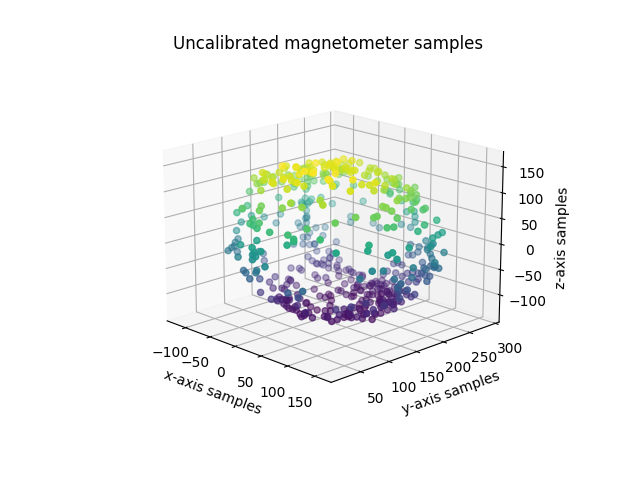
\includegraphics[width=\textwidth]{unclibrated-mag.png}
        \caption{Uncalibrated magnetometer samples}
        \label{fig:uncalibrated}
    \end{subfigure}
    \hfill
    \begin{subfigure}[!h]{0.49\textwidth}
        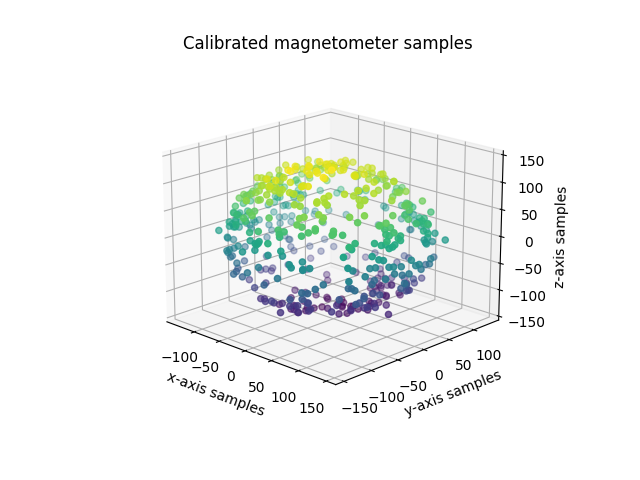
\includegraphics[width=\textwidth]{calibrated-mag.png}
        \caption{Calibrated magnetometer samples}
        \label{fig:calibrated}
    \end{subfigure}
    \caption{Calibration process}
    \label{fig:calibration}
\end{figure}



\subsection{Digital filter}
After calibrating the digital compass and applying tilt-compensation, measurement noise was found to be present on the samples taken. A discrete second order Butterworth LPF was thus implemented to 
reduce the measurement noise. The filter parameters were determined using Scipy.signal.butter(), in Python. Different cutt-off frequencies for the filter were experimented with, the cutt-off frequency 
that produced minimal deviation on the output of the signal, as well as sufficiently low response time to a step input was chosen. 

Five hundred samples were taken with at a sample period of 70 ms, the digital compass was placed on a flat surface with a heading of $90^{\circ}$ (verified by the handheld magnetic compass). The mean
value of the samples was $89.634^{\circ}$, and variation from the mean was found to be $7.747^{\circ}$. To determine the optimal cutt-off frequency of the LPF filter, the filter was applied to the
samples, each time with a different cutt-off frequency, and the resulting deviation at the output was measured. To determine the response time of the filter to varying cutt-off frequencys, five 
hundred samples were again taken, but this time the digital compass was rotated $90^{\circ}$ during sampling to produce a step input for the filter, response times were then measured to this step input.
The reulting deviation at the output and response times for the varying cutt-off frequencies is shown in table\ref{table:filter}. The cutt-off frequency is shown in the discrete domain, therefore to 
determine the corresponding frequency in the continuous time domain simply multiply by the sampling frequency, which is 14.286 Hz.

\begin{table}[!h]
    \centering
    \caption{Response time and deviation for different LPF cutt-off frequencies}
    \label{table:filter}
    \begin{tabularx}{\columnwidth}{ | X | X | X | }
        
        \hline
        Cutt-off frequency & Response time (ms) & Variance (degrees)\\
        \hline
        0.3 &  137 & 4.0512 \\
        \hline
        0.25 &  161 & 3.4841 \\
        \hline
        0.2 &  234 & 2.9346 \\
        \hline
        0.15 &  363 & 2.3633 \\
        \hline
        0.12 &  492 & 2.1912 \\
        \hline
        0.1 &  630 & 1.7741 \\
        \hline
        0.05 &  1282 & 1.0558 \\
        \hline
    \end{tabularx}
\end{table}

A cutt-off frequency of 0.12 rad/sample was chosen as it corresponds to a response time of under 500 ms, and a sufficiently low deviation on the output. Fast response time is important in 
this specific application in order to correct the heading of the vessel quickly, should it go off course.

The transfer function of a discrete second-order Butterworth LPF is shown in Eq.\ref{eq:filter_tf}. The parameters found for a cutt-off frequency of 0.12 rad/sample are shown in 
Eq.\ref{eq:filter_b} and Eq.\ref{eq:filter_a}

\begin{equation}
    \label{eq:filter_tf}
    Y(z) = \left( \frac{b_{0} + b_{1}z^{-1} + b_{2}z^{-2}}{a_{0} + a_{1}z^{-1} + a_{2}z^{-2}} \right) \cdot X(z)
\end{equation}


\begin{equation}
    \label{eq:filter_b}
    b = (0.02785977, 0.05571953, 0.02785977) 
\end{equation}


\begin{equation}
    \label{eq:filter_a}
    a = (1. , -1.47548044, 0.58691951)
\end{equation}

The LPF filter is then implemented in software as a difference equation shown in Eq.\ref{eq:filter_code}. The filter was applied to the raw magnetometer and raw accelerometer samples (raw means 
before tilt-compensation is applied), this was done to avoid a erronous heading being returned that occurs when samples cross back and forth over $0^{\circ}$. Applying
the filter to the accelerometer samples will reduce signal noise caused by high frequency vibrations that occur during a jybe manouvre, due to the sail swapping over.


\begin{equation}
    \label{eq:filter_code}
    y[n] = \frac{b_{0}x[n] + b_{1}x[n-1] + b_{2}x[n-2] - a_{1}y[n-1] - a_{2}y[n-2]}{a_{0}}
\end{equation}


The output of the digital LPF filter designed using a cutt-off frequency of 0.12 rad/sample is shown in Fig.\ref{fig:lpf_output}, and the step response to a $90^{\circ}$ step change is shown in
Fig.\ref{fig:filter_step}.

\begin{figure}[!h]
    \centering
    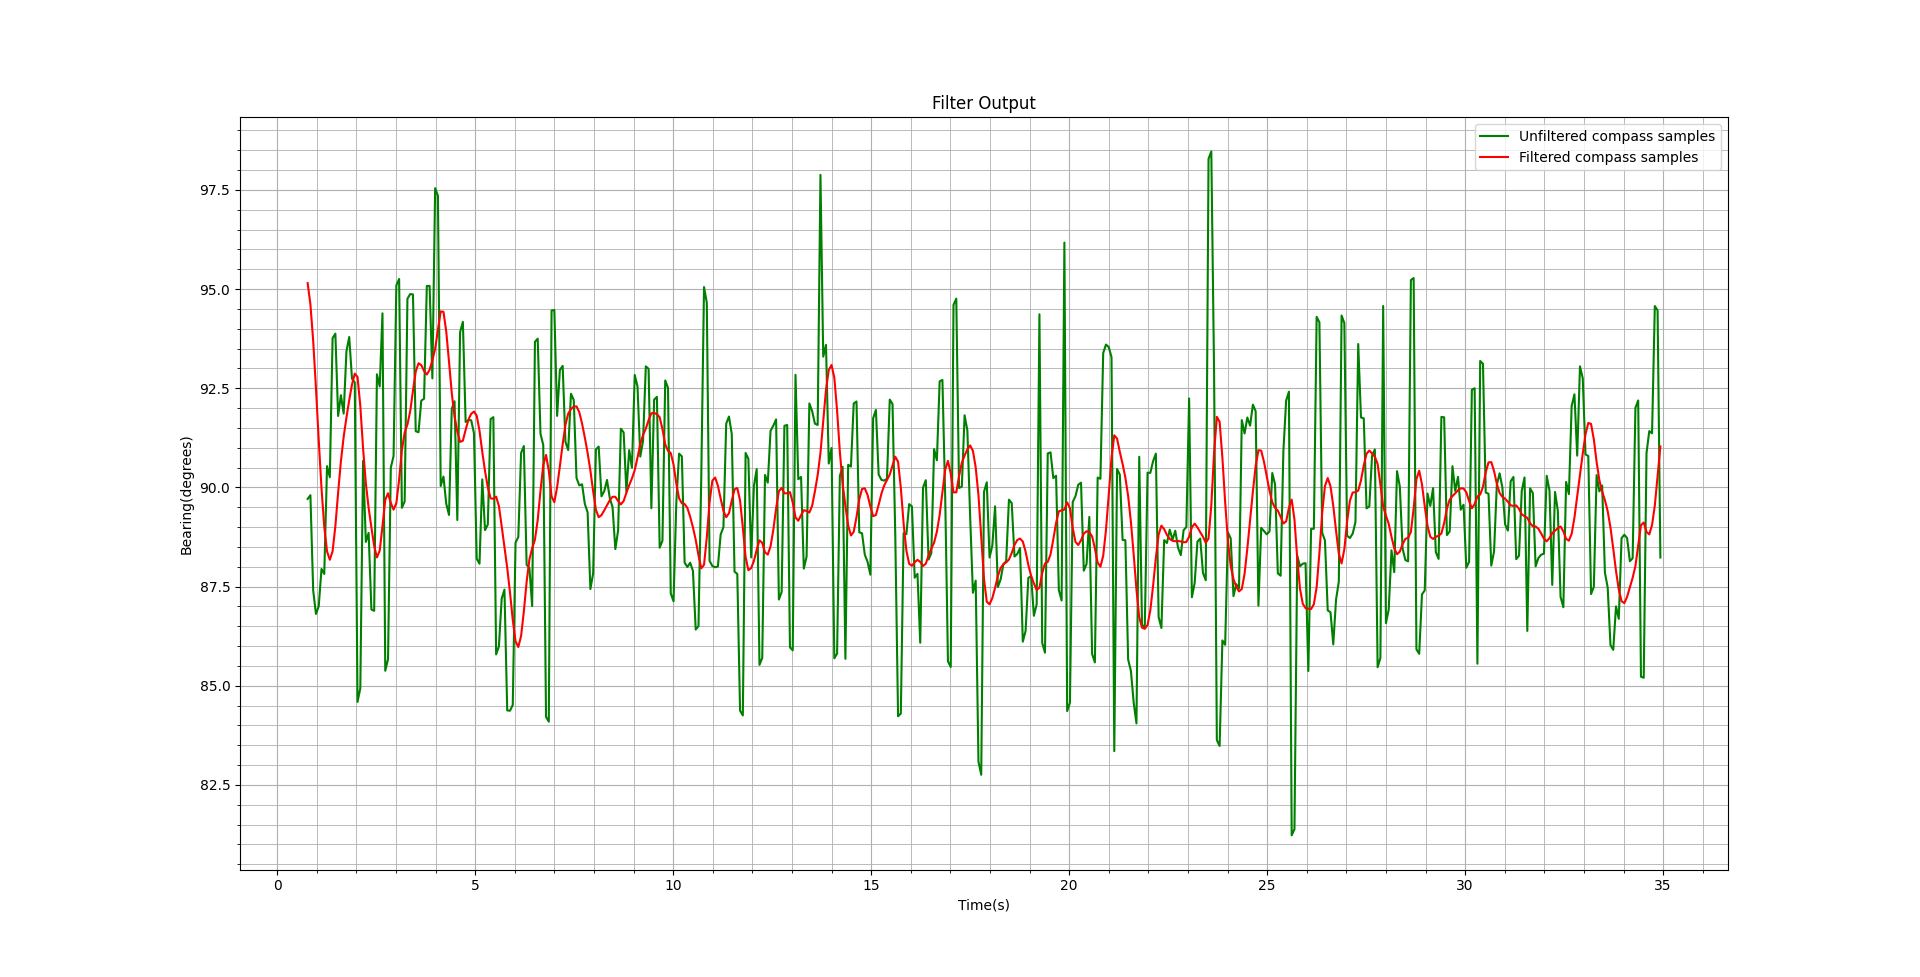
\includegraphics[width=0.98\linewidth]{Filter_output.png}
    \caption[Digital compass discrete LPF output]{Discrete LPF output}
    \label{fig:lpf_output}
\end{figure}

\begin{figure}[!h]
    \centering
    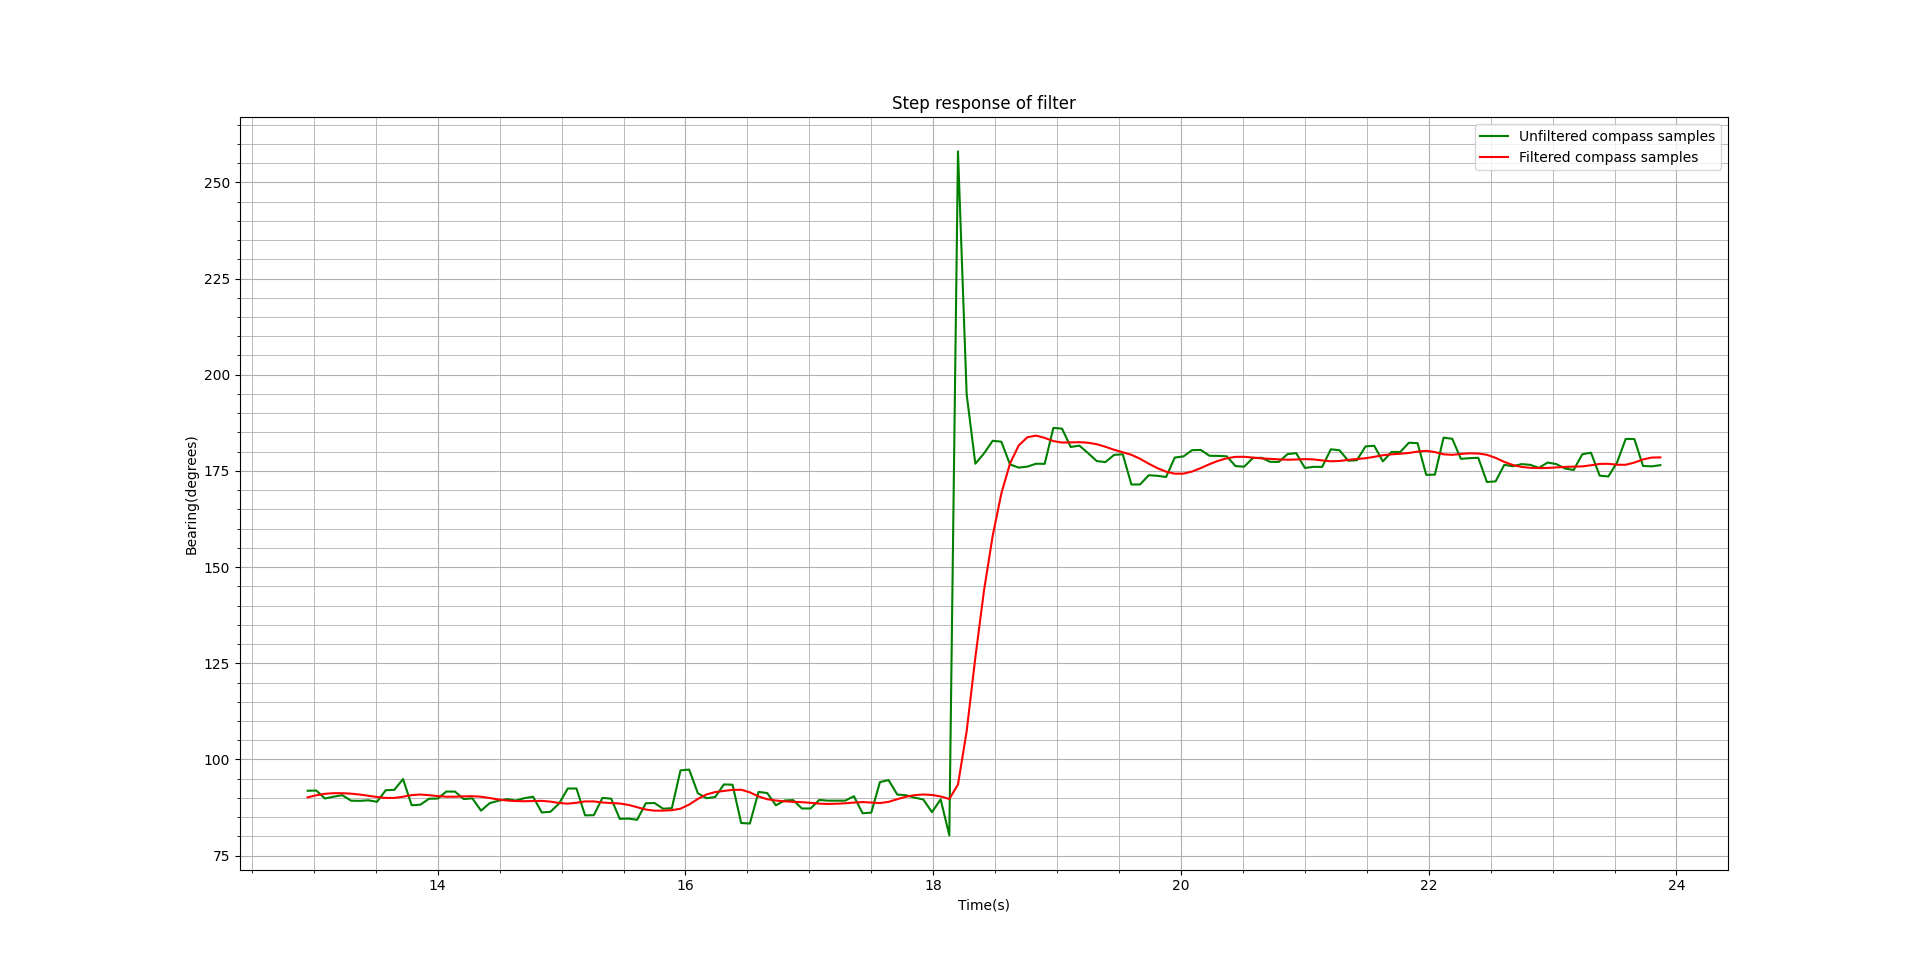
\includegraphics[width=0.98\linewidth]{Step_response.png}
    \caption[Digital compass discrete LPF step response]{Discrete LPF step response}
    \label{fig:filter_step}
\end{figure}

\section{Power System}
%Must still measure current draw of servo motors
The Adafruit feather consumes a maximum of 80 mA when operating, the MPU-9250/6500 consumes 3.7 mA, the GPS receiver consumes 100 mA and the SD card uses 30 mA when writing or reading data. The
data-sheet for the FST200-202 does not specify power consumption, the maximum current draw was however measured to be 34.2 mA. The overall current draw of the system is therefore 247,9 mA. A 
9V Duracell battery has a milli-amp hour capacity of 310 mAh at 100 mA discharge\cite{mah}. If two 9V batteries connected in series are used to power the entire system, then the battery life will 
be less than 1,25 hours. If the two 9V batteries are used to power the wind sensor only, their life will be expanded to roughly 9,064 hours. The decision was therefore made to use the two 9V batteries to power the 
wind sensor alone, and have a separate power source for the micro-controller, GPS module, digital compass and SD card. A 5000mAh 3.7V lithium polymer battery was used to power the Adafruit feather
board. The feathers 3.3V regulator was then used to power the GPS receiver, MPU-9250/6500 IMU and SD card. The Adafruit feathers datasheet specifies that the 3.3V regulator is capable of deliverin
500 mA peak (not continuous)\cite{feather}. The combined current draw of the GPS receiver, MPU-9250/6500 IMU and SD card is 133,7 mA, which is much lower than the peak specification. The decision was made
to use the power source already present in the RC sailboat to power the two servo motors. The RC sailboat was designed to operate with a 6V power source (four 1.5V
alkaline batteries in series) for the two servo motors.  

\section{PCB}
A printed circuit board was designed using Altium Designer and printed with a LPKF 62 routing machine. The PCB was designed for the Adafruit feather, the GPS receiver, the MPU-9250/6500 and the 
micro-SD card socket. The PCB has input pins for the 3.7V lithium polymer battery and the 18V power source, the wind sensor connects to the board via a screw terminal and the two servo motors
connect to the board with dedicated pins. A power plane was used to distribute ground potential to all the components. The PCB has only one side of copper plating. Component schematics and footprints
were made from scratch. Fig.\ref{fig:pcb} shows a schematic of the PCB design, the system diagram used to generate the PCB schematic can be found in appendix\ref{appen:system}.

\begin{figure}[!h]
    \centering
    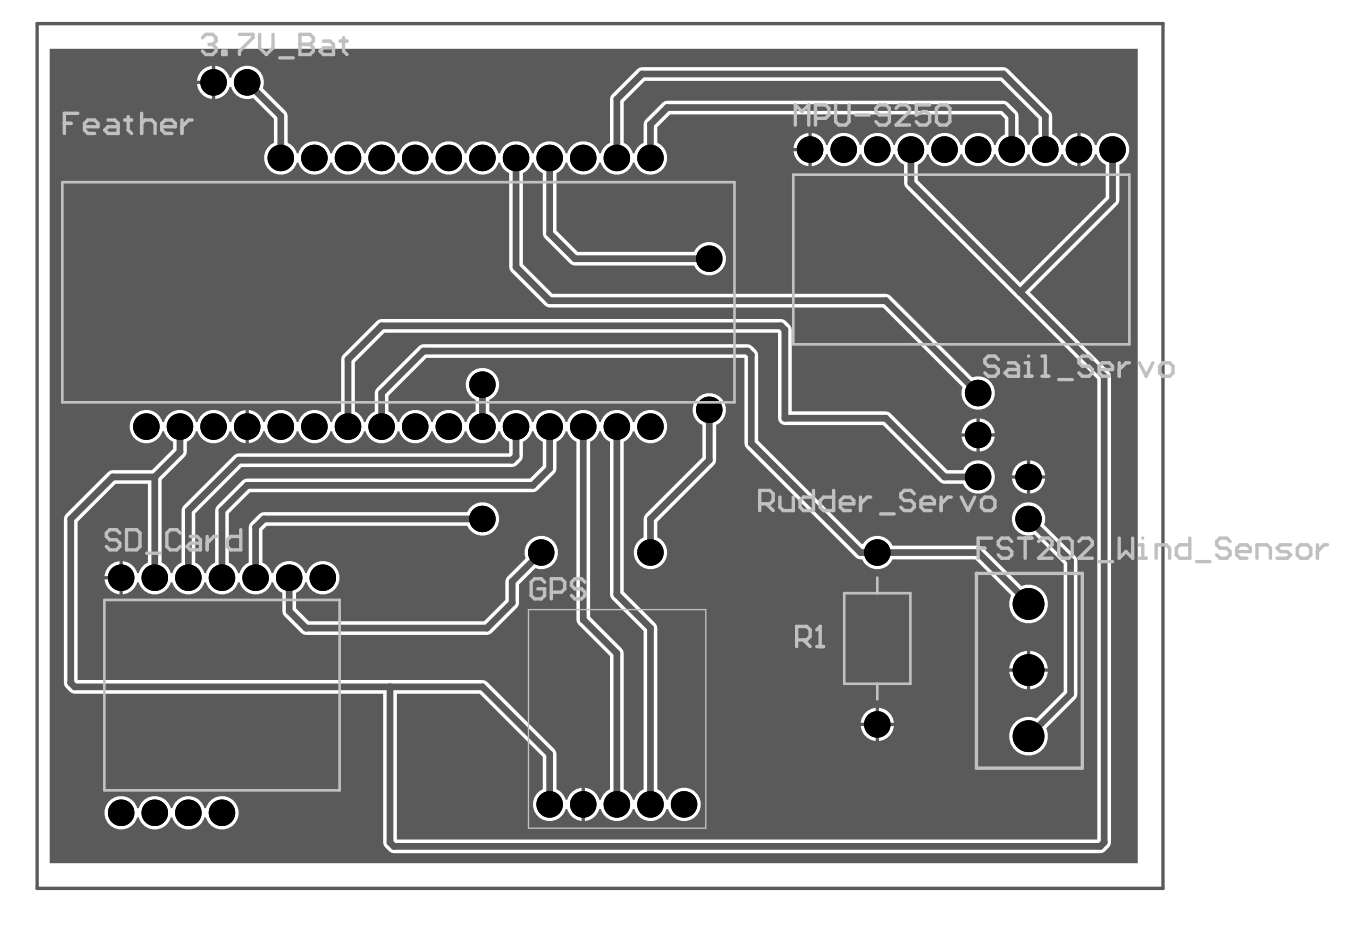
\includegraphics[width=0.8\linewidth]{system_pcb.png}
    \caption[PCB schematic]{PCB schematic}
    \label{fig:pcb}
\end{figure}



\section{Software}

\subsection{Control systems}
The control systems of the vessel consist of the rudder controller and the sail controller. Fig.\ref{fig:control-system} isllustrates the architecture of the control system. The reference signal
for the system is the heading between the current GPS-coordinates and the target GPS-coordinates, the actual heading (measured with the digital compass) is subtracted from the reference heading
to create the error signal for the rudder controller. The rudder controller then controls the rudder actuator (servo motor). 
The wind direction sensor determines apparent wind direction, this 
is then input to the sail controller, which adjusts the sail position with a control signal sent to the sail actuator.

\begin{figure}[!h]
    \centering
    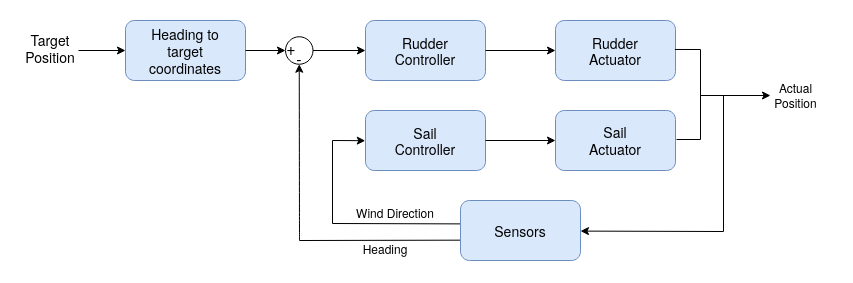
\includegraphics[width=0.98\linewidth]{control_system.png}
    \caption[Control system]{control system}
    \label{fig:control-system}
\end{figure}


\subsubsection{Sail controller}

The ADC that samples the wind direction sensors output returns a value in the range of 0 to $2^{16}$. Table \ref{table: ...} shows the minimum and maximum voltage values measured at the output of 
the sensor and the corresponding sampled ADC values expressed as a percentage. 

\begin{table}[!h]
    \centering
    \caption{Wind direction sensor output limits}
    \label{table:adc-limits}
    \begin{tabularx}{\columnwidth}{ | X | X | X | }
        
        \hline
         &Measured Voltage & ADC sampled value (\%)\\
        \hline
        Minimum & 642mV & 19.63\%  \\
        \hline
        Maximum & 3.07V & 93.1152\%  \\
        \hline
    \end{tabularx}
\end{table}

Eq.\ref{eq:sail-control-alpha} is implemented to remove the 642mV offset and convert the sampled ADC value to a value in the range $0^{\circ}$ to $360^{\circ}$. This value therefore represents the
direction of apparent wind. The cross-over point is the point where the voltage output of the sensor changes from a maximum to a minimum i.e. the voltage drops from 3.07V to 642mV. This drop does 
not occur instantaneously and because of this erronous readings can occur if samples are taken at the cross-over point. The controller was therefore designed with the wind sensor orientated such that 
the cross-over point lies in the no-sail zone, as readings taken in this area are not used anyway.


\begin{equation}
    \label{eq:sail-control-alpha}
    \alpha = \left( \frac{ADC_{sample} - ADC_{min}}{ADC_{max} - ADC_{min}} \right) \cdot 360^{\circ}
\end{equation}


When designing the sail controller the limits of the sail vessel must be taken into account i.e. the no sail zone. The sail position must be at $10^{\circ}$ when the apparent wind is $\pm 45^{\circ}$,
and sail position must be at $80^{\circ}$ when apparent wind is at $\pm 180^{\circ}$. Eq.\ref{eq:sail-control-algorithm} implements these requirements using PWM maximum and minimum values measured and recorded in table
\ref{table:pwm}. The duty cycle of the PWM signal used for the sail servo winch is stored in a 16 bit register, and is set using Eg.\ref{eq:duty_cycle}.

\begin{equation}
    \label{eq:sail-control-algorithm}
    PWM_{val} = \left( \frac{\alpha - 45^{\circ}}{180^{\circ} - 45^{\circ}} \right) \cdot \left( PWM_{max} - PWM_{min}\right) + PWM_{min}
\end{equation}

\begin{equation}
    \label{eq:duty_cycle}
    duty\_cycle = \left(\frac{PWM\_value}{1000}\right) \cdot 2^{16}
\end{equation}


\subsubsection{Rudder Controller}
%Just using proportional control for now  
The rudder controller can be designed through simulation, using the methods described in subsection \ref{sec:robotics-paper}, or by adjustment through experimentation. To design a rudder 
controller using simulation methods, the dynamics of the sail vessel need to be determined, which is not a trivial task. Eq.\ref{eq:sail_dynamics} is used to calculate and model the dynamics 
of a sail vessel, and involves calculating hydrodynamics, moment of inertia, viscous damping, lift, effort sail and centre of mass. From results in subsection \ref{sec:robotics-paper}, 
it is clear that the controller parameters determined through simulation were not optimal and therefore of design rudder controller for this project is done by adjustment.

The rudder controller used is a proportional controller. The control law for this controller is shown in Eq.\ref{eq:control-law}, where $k_{p}$ is the proportional gain and $E_{r}$ is the 
error signal. The error signal is determined using Eq.\ref{eq:error-sig}, where $\psi_{r}$ is the reference bearing and $\psi_{a}$ is the actual bearing of the vessel. 

\begin{equation}
    \label{eq:control-law}
    U[k] = k_{p}E_{r}
\end{equation}

\begin{equation}
    \label{eq:error-sig}
    E_{r} = \psi_{r} - \psi_{a}
\end{equation}

After calculating the error signal a check is done in software: if the error signal is greater than $180^{\circ}$ then subtract $360^{\circ}$, and if the error signal is smaller than $180^{\circ}$
then add $360^{\circ}$, else do nothing. This check is done to ensure that the vessel turns in the direction associated with the smallest angle of correction. For example: if the angle of correction
in the clockwise direction is $100^{\circ}$ and $60^{\circ}$ in the anti-clockwise direction, the boat will turn anti-clockwise.

Eq.\ref{eq:pwm-sig-rudder} is used to determine the duty cycle - Eq.\ref{eq:duty_cycle} - of the PWM signal that controls the rudder servo. The maximum and minimum PWM values measured in table \ref{table:pwm}
are used here.

\begin{equation}
    \label{eq:pwm-sig-rudder}
    PWM_{val} = \left( \frac{U[k]}{60^{\circ}} \right) \cdot (PWM_{max} - PWM_{min}) + \left( \frac{PWM_{max} + PWM_{min}}{2} \right)
\end{equation}

\subsection{Navigational calculations}
\subsubsection{Distance}
To calculate distance over the surface of a sphere two options were considered: The Haversine formulae and the equirectangular approximation. The Haversine formulae is more accurate but can be 
computationally expensive, the equirectangular approximation is less accurate but more efficient. The Haversine formulae was chosen as the accuracy is required. The Haversine formulae is shown 
in Eq.\ref{eq:haversine1} and Eq.\ref{eq:haversine2}, where
the current coordinates are $(lat_1, long_1)$ and the target coordinates are $(lat_2, long_2)$, R is the radius of the earth in km. Coordinates are in decimal degrees.

\begin{equation}
    \label{eq:haversine1}
    a = sin^{2}\left( \frac{lat_{2} - lat_{1}}{2}\right) + cos(lat_{1})\cdot cos(lat_{2})\cdot sin^2\left(\frac{long_{2} - long_{1}}{2}\right)
\end{equation}

\begin{equation}
    \label{eq:haversine2}
    d = R\cdot \left(2\arctan\left(\frac{\sqrt{a}}{\sqrt{1-a}}\right)\right)
\end{equation}


Eq.\ref{eq:haversine1} returns values in the order of $e-17$ for a 
distance on 1m. In Python floats are single precision numbers with a maximum value of $\pm3.4e38$ and minimum value of $\pm1.7e-38$, therefore the haversine function can be used to determine 
small distances on the micro-controller. 

\subsubsection{Heading}
To calculate reference heading Eq.\ref{eq:ref-heading} is used.

\begin{equation}
    \label{eq:ref-heading}
    \psi_{r} = \arctan\left( \frac{sin(long_2 - long_1)cos(lat_2)}{cos(lat_1)sin(lat_2) - sin(lat_1)cos(lat_2)cos(long_2 - long_1)}\right)
\end{equation}


\subsection{Program flow}



\graphicspath{{conclusion/fig/}}

\chapter{Summary and Conclusion}
\label{chap:conclusion}

% Bibliography
\bibliography{mybib}

% End matter
\appendix
\graphicspath{{appendices/fig/}}

\chapter{System schematic}
\makeatletter\@mkboth{}{Appendix}\makeatother
\label{appen:system}

\begin{figure}[!h]
    \centering
    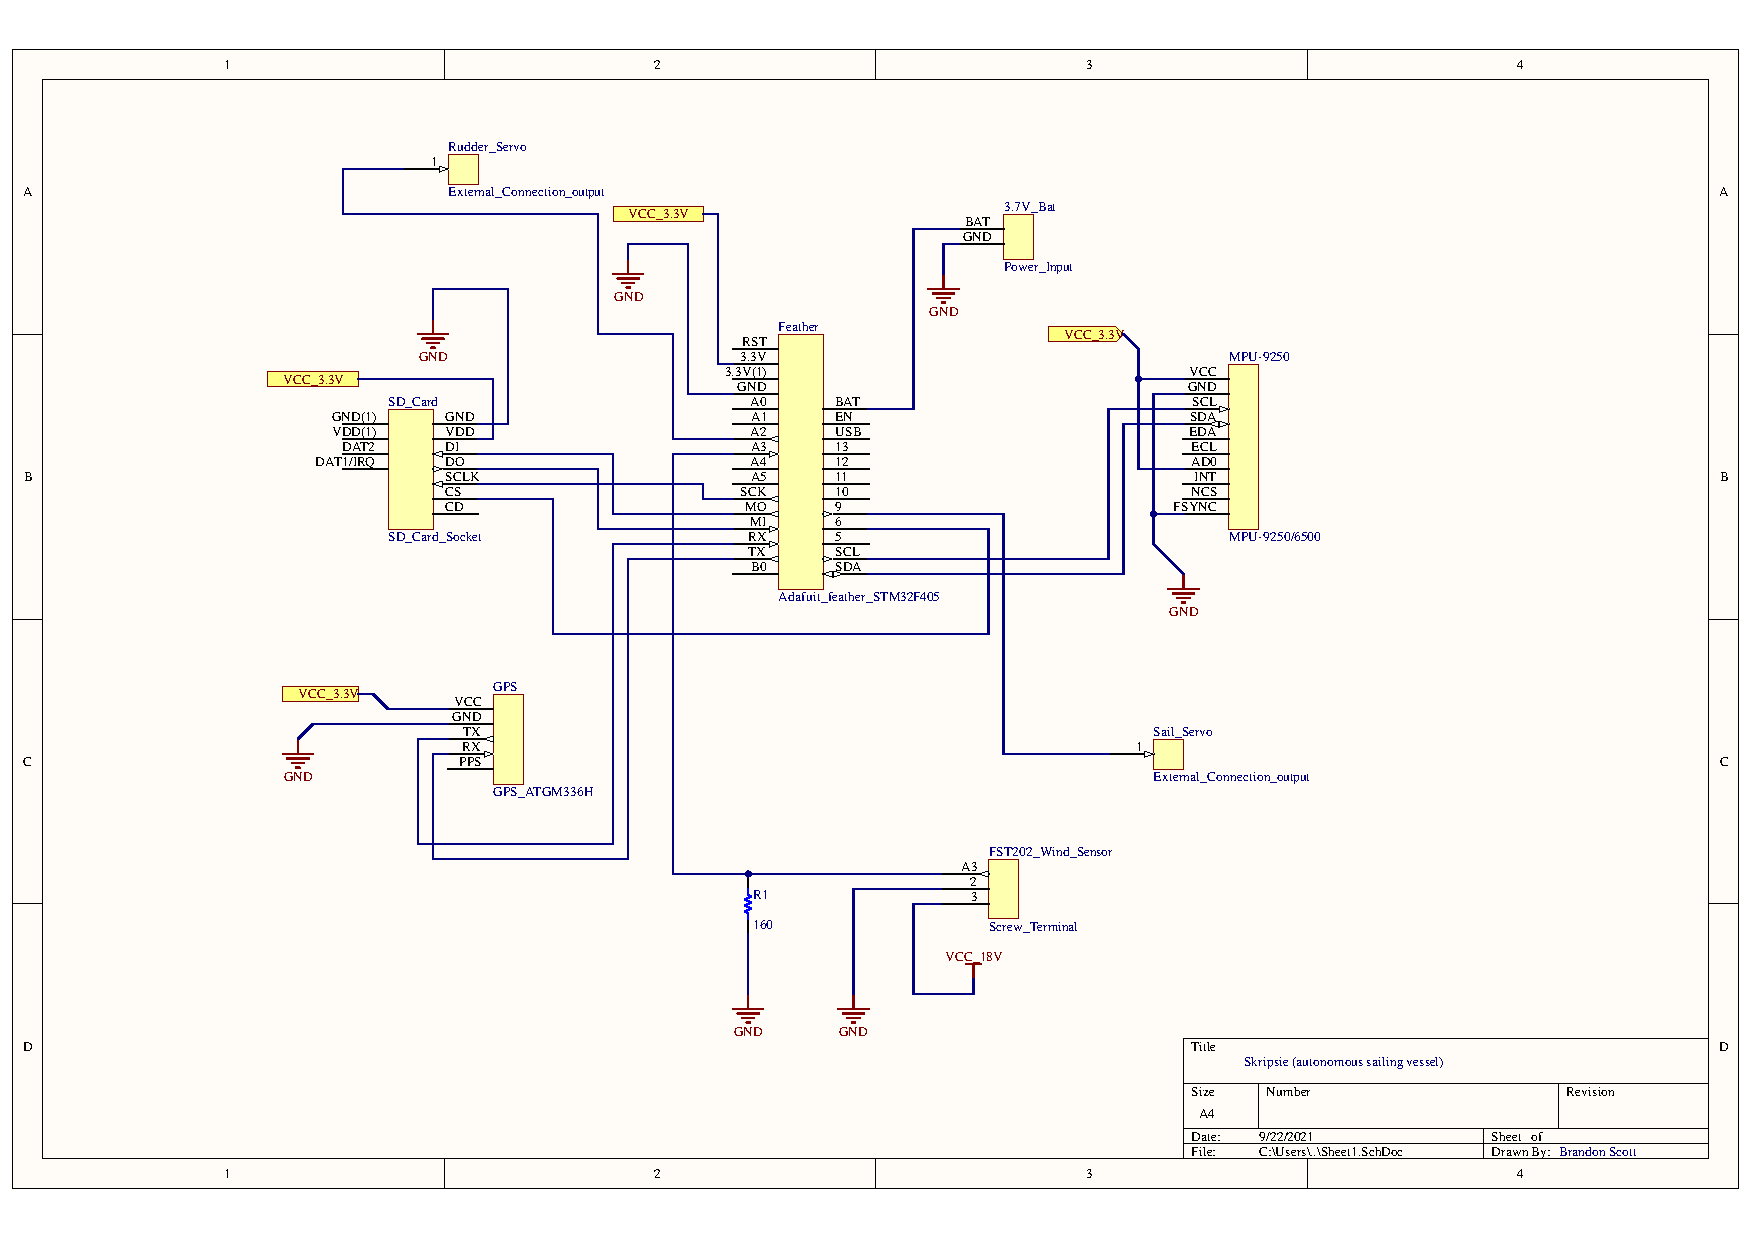
\includegraphics[angle=90,width=0.8\linewidth]{Skripsie-1.pdf}
\end{figure}


\end{document}

